% Why do we need to submit this? It's not part of the markscheme and you wouldn't
% usually give out your TeX code, just the PDF.

% -------------------------------------------------------------------------------
% Establish page structure & font.
\documentclass[12pt]{report}\usepackage[]{graphicx}\usepackage[]{xcolor}
% maxwidth is the original width if it is less than linewidth
% otherwise use linewidth (to make sure the graphics do not exceed the margin)
\makeatletter
\def\maxwidth{ %
  \ifdim\Gin@nat@width>\linewidth
    \linewidth
  \else
    \Gin@nat@width
  \fi
}
\makeatother

\definecolor{fgcolor}{rgb}{0.345, 0.345, 0.345}
\newcommand{\hlnum}[1]{\textcolor[rgb]{0.686,0.059,0.569}{#1}}%
\newcommand{\hlstr}[1]{\textcolor[rgb]{0.192,0.494,0.8}{#1}}%
\newcommand{\hlcom}[1]{\textcolor[rgb]{0.678,0.584,0.686}{\textit{#1}}}%
\newcommand{\hlopt}[1]{\textcolor[rgb]{0,0,0}{#1}}%
\newcommand{\hlstd}[1]{\textcolor[rgb]{0.345,0.345,0.345}{#1}}%
\newcommand{\hlkwa}[1]{\textcolor[rgb]{0.161,0.373,0.58}{\textbf{#1}}}%
\newcommand{\hlkwb}[1]{\textcolor[rgb]{0.69,0.353,0.396}{#1}}%
\newcommand{\hlkwc}[1]{\textcolor[rgb]{0.333,0.667,0.333}{#1}}%
\newcommand{\hlkwd}[1]{\textcolor[rgb]{0.737,0.353,0.396}{\textbf{#1}}}%
\let\hlipl\hlkwb

\usepackage{framed}
\makeatletter
\newenvironment{kframe}{%
 \def\at@end@of@kframe{}%
 \ifinner\ifhmode%
  \def\at@end@of@kframe{\end{minipage}}%
  \begin{minipage}{\columnwidth}%
 \fi\fi%
 \def\FrameCommand##1{\hskip\@totalleftmargin \hskip-\fboxsep
 \colorbox{shadecolor}{##1}\hskip-\fboxsep
     % There is no \\@totalrightmargin, so:
     \hskip-\linewidth \hskip-\@totalleftmargin \hskip\columnwidth}%
 \MakeFramed {\advance\hsize-\width
   \@totalleftmargin\z@ \linewidth\hsize
   \@setminipage}}%
 {\par\unskip\endMakeFramed%
 \at@end@of@kframe}
\makeatother

\definecolor{shadecolor}{rgb}{.97, .97, .97}
\definecolor{messagecolor}{rgb}{0, 0, 0}
\definecolor{warningcolor}{rgb}{1, 0, 1}
\definecolor{errorcolor}{rgb}{1, 0, 0}
\newenvironment{knitrout}{}{} % an empty environment to be redefined in TeX

\usepackage{alltt}

\usepackage[a4paper, margin=3cm]{geometry} % Page structure

\usepackage{graphicx} % Required for inserting images
\graphicspath{{images/}} % Any additional images I use (BCU logo, etc) are from here.

\usepackage[utf8]{inputenc} % UTF-8 encoding
\usepackage[T1]{fontenc} % T1 font
\usepackage{float}  % Allows for floats to be positioned using [H], which correctly
                    % positions them relative to their location within my LaTeX code.
\usepackage{subcaption}

% -------------------------------------------------------------------------------
% Declare biblatex with custom Harvard BCU styling for referencing.
\usepackage[
    useprefix=true,
    maxcitenames=3,
    maxbibnames=99,
    style=authoryear,
    dashed=false, 
    natbib=true,
    url=false,
    backend=biber
]{biblatex}

% Additional styling options to ensure Harvard referencing format.
\renewbibmacro*{volume+number+eid}{
    \printfield{volume}
    \setunit*{\addnbspace}
    \printfield{number}
    \setunit{\addcomma\space}
    \printfield{eid}}
\DeclareFieldFormat[article]{number}{\mkbibparens{#1}}

% Declare report.bib as the bibliography source, to be called later via \printbibliography
\addbibresource{report.bib}

% Also import hyperref, used for embedding URLs.
\usepackage{hyperref}

% Set certain colours up for links, whether they link to within the document (citations, contents page)
% or to an external resource (websites)
\hypersetup{
    colorlinks=true,
    linkcolor=black, % Contents page
    urlcolor=blue, % URLs
    citecolor=black, % Citations
}

% -------------------------------------------------------------------------------
% To prevent "Chapter N" display for each chapter
\usepackage[compact]{titlesec}
\usepackage{wasysym}
\usepackage{import}

\titlespacing*{\chapter}{0pt}{-2cm}{0.5cm}
\titleformat{\chapter}[display]
{\normalfont\bfseries}{}{0pt}{\Huge}

% -------------------------------------------------------------------------------
% Custom macro to make an un-numbered footnote.

\newcommand\blfootnote[1]{
    \begingroup
    \renewcommand\thefootnote{}\footnote{#1}
    \addtocounter{footnote}{-1}
    \endgroup
}

% -------------------------------------------------------------------------------
% Fancy headers; used to show my name, BCU logo and current chapter for the page.
\usepackage{fancyhdr}
\usepackage{calc}
\pagestyle{fancy}

\setlength\headheight{37pt} % Set custom header height to fit the image.

\renewcommand{\chaptermark}[1]{%
    \markboth{#1}{}} % Include chapter name.


% Lewis Higgins - ID 22133848           [BCU LOGO]                [CHAPTER NAME]
\lhead{Lewis Higgins - ID 22133848~~~~~~~~~~~~~~~
\includegraphics[width=1.75cm]{bcu logo}}
\fancyhead[R]{\leftmark}


% -------------------------------------------------------------------------------
%TC:envir knitrout* [ignore] knitrout
% -------------------------------------------------------------------------------

\title{Visualising Trends in Apps on the Google Play Store}
\author{Lewis Higgins - Student ID 22133848}
\date{May 2024}

% -------------------------------------------------------------------------------
\IfFileExists{upquote.sty}{\usepackage{upquote}}{}
\begin{document}





\makeatletter
\begin{titlepage}
    \begin{center}
        
\includegraphics[width=0.7\linewidth]{bcu logo}\\[7ex]
        {\huge \bfseries  \@title }\\[30ex]
        {\@author}\\[2ex]
        {CMP5352 - Data Visualisation}\\[10ex]
        {Word count of RNW file (excluding code, figures, and tables): 3299}\\[10ex]
    \end{center}
\end{titlepage}
\makeatother
\thispagestyle{empty}
\newpage

\begin{abstract}

    This report delves into a dataset containing information
    on a wide variety of apps from the Google Play Store. 
    By leveraging Exploratory Data Analysis (EDA) and data visualization techniques, 
    the report aims to uncover insights and trends within 
    the Play Store ecosystem based on data such as review scores, install counts and app
    categories.

\end{abstract} 

% Page counter trick so that the contents page doesn't increment it.
\setcounter{page}{0}

\tableofcontents
\thispagestyle{empty}

% Declaring un-numbered chapter because I prefer how it looks.
\chapter*{Introduction}
% Add it to the contents, because un-numbered chapters aren't by default.
\addcontentsline{toc}{chapter}{Introduction}
% Put the chapter name in the header.
\markboth{Introduction}{}

Data visualisation is a field of data science wherein large datasets are parsed
using code (most commonly written in Python or R) to produce clear visualisations
interpretable to a wide audience, even if they do not have in-depth knowledge
of the dataset. \\

\noindent This report specifically aims to produce visualisations based on an
analysis of a large dataset based on the content available on the Google Play Store, 
where users of Android mobile devices can download a wide variety of apps to suit their needs. 
The mobile app industry is an enormous market to be involved in, with over 27 billion 
downloads occurring on the Play Store in Q1 2023 alone \autocite{PlayStoreDLs}. This report delves 
into a comprehensive dataset of apps available on the Play Store, aiming to uncover valuable insights 
and trends. Through exploratory data analysis, the composition of the store will 
be examined, including factors such as app reviews in comparison to their install counts, as well as 
additional insights such as app pricing and how it affects user counts.
This exploration will also provide potential indicators of current and future trends within the Play Store
and the broader mobile market.\\



\noindent This report is split across three sections:
\begin{itemize}
    \item The \textbf{motivation and objectives} of this report.
    \item The \textbf{results from experiments} on the dataset.
    \item A \textbf{summary} of overall findings.
\end{itemize}

\noindent This report was compiled as a .Rnw file, meaning that all R code used in this
report is embedded into the PDF and readable within the report. A webapp where data can 
be generated from the dataset is attached with this PDF within the "Shiny" folder.

\pagebreak

\chapter{Motivation and objectives}

% Put the chapter name in the header.
\markboth{Motivation and objectives}{}

The Google Play Store is a massive market to tap into, hosting over 3.5 million apps as of Q3 2022 
\autocite{PlayStoreAppCount}, so it is therefore crucial to understnad current and future trends
to ensure that content released on the store can be properly optimised to maximise install count and 
review scores, which will ultimately increase profit.\\

\noindent The dataset used is \href{https://www.kaggle.com/datasets/lava18/google-play-store-apps/data}{sourced from Kaggle}, a 
public dataset-sharing website. It contains 9660 unique values with 13 columns of data:

\begin{itemize}
    \item App - The name of the app.
    \item Category - The specific category of the app.
    \item Rating - A number between 1 and 5, representing the "star" rating of the app.
    \item Reviews - The amount of reviews for the app.
    \item Size - The size of the app in kilobytes or megabytes.
    \item Installs - Number of user installs of the app.
    \item Type - Whether the app costs money or is free.
    \item Price - The price of the app in dollars, or 0 if it is free.
    \item Content.Rating - The general age rating of the app.
    \item Genres - The genres associated with the app.
    \item Last.Updated - The most recent date when the app received an update.
    \item Current.Ver - The version number of the app.
    \item Android.Ver - The required Android version of the app.
\end{itemize}
\pagebreak
\section{Key questions and expected answers conerning the data}\label{sec:questions} % For later reference
\begin{itemize}
    \item Is there a positive correlation between the average review score of an app and its install count? 
    \begin{itemize}
        \item Expected: Yes, as it is harder to weigh the average down when the volume of installs increases.
    \end{itemize}
    \item Which category of app has the highest review score on average?
    \begin{itemize}
        \item Expected: Games are likely to have the highest review scores from users enjoying their experiences.
    \end{itemize}
    \item What is the distribution of prices? Are there certain prices used by many apps?
    \begin{itemize}
        \item Expected: If an app is not free, it would likely be under \$3 to ensure people buy it.
    \end{itemize}
    \item Do paid apps receive higher or lower review score on average?
    \begin{itemize}
        \item Expected: No, as users may be more harsh with their reviews if they paid for the app.
    \end{itemize}
    \item Is there a correlation between an app's content rating and it's review score?
    \begin{itemize}
        \item Expected: Yes, with adult apps likely being higher rated because children would be unlikely to have accounts.
    \end{itemize}
    \item Does app size play a role in install count?
    \begin{itemize}
        \item Expected: Yes, as users would likely not want to download very large apps due to internet speeds and device storage.
    \end{itemize}
\end{itemize}

\pagebreak

\chapter{Experimental results}

% Put the chapter name in the header.
\markboth{Experimental results}{}



\section{Data wrangling}
To be able to analyse the data, it is essential that the data is first in a state that
can be analysed effectively. To do so, the data must be explored to identify any potential
issues, and any that are found must be cleaned, which is referred to as data wrangling. This 
process is vital to ensure that any products of this data are accurate, correct and not misleading
to viewers as a result of incomplete or inconsistent data.\\

\noindent Another good step to take in the initial exploration of the data is to identify if there are any missing values
in certain columns. To do so, we can convert any instance of a blank string into R's recognised "NA" type and
then use is.na() to identify how many there are.

\begin{knitrout}
\definecolor{shadecolor}{rgb}{0.969, 0.969, 0.969}\color{fgcolor}\begin{kframe}
\begin{alltt}
\hlcom{# Convert blank strings or NaN to NA.}
\hlstd{dataDf[(dataDf} \hlopt{==} \hlstr{""} \hlopt{|} \hlstd{dataDf} \hlopt{==} \hlstr{"NaN"}\hlstd{)]} \hlkwb{<-} \hlnum{NA}

\hlcom{# Identify rows containing NA.}
\hlstd{naRows} \hlkwb{<-} \hlstd{dataDf[}\hlkwd{rowSums}\hlstd{(}\hlkwd{is.na}\hlstd{(dataDf)} \hlopt{>} \hlnum{0}\hlstd{),]}
\hlkwd{nrow}\hlstd{(naRows)}
\end{alltt}
\begin{verbatim}
[1] 1481
\end{verbatim}
\begin{alltt}
\hlkwd{nrow}\hlstd{(naRows)}\hlopt{/}\hlkwd{nrow}\hlstd{(dataDf)}\hlopt{*}\hlnum{100}
\end{alltt}
\begin{verbatim}
[1] 13.66
\end{verbatim}
\end{kframe}
\end{knitrout}

We can identify that this dataset has 1481 rows where at least one column has missing data, equating to 
13.66\% of the dataset. To analyse this in further detail,
the naniar package can be used to generate a tibble of where the data is missing.

\begin{knitrout}\footnotesize
\definecolor{shadecolor}{rgb}{0.969, 0.969, 0.969}\color{fgcolor}\begin{table}[H]
\centering
\caption{\label{tab:missingVars}Missing variable summary of the dataset}
\centering
\begin{tabular}[t]{l|r|r}
\hline
variable & n\_miss & pct\_miss\\
\hline
Rating & 1474 & 13.6\\
\hline
Current.Ver & 8 & 0.0738\\
\hline
Android.Ver & 3 & 0.0277\\
\hline
Type & 1 & 0.00922\\
\hline
Content.Rating & 1 & 0.00922\\
\hline
App & 0 & 0\\
\hline
Category & 0 & 0\\
\hline
Reviews & 0 & 0\\
\hline
Size & 0 & 0\\
\hline
Installs & 0 & 0\\
\hline
Price & 0 & 0\\
\hline
Genres & 0 & 0\\
\hline
Last.Updated & 0 & 0\\
\hline
\end{tabular}
\end{table}

\end{knitrout}

% unique(dataDf$rating)

    
\begin{knitrout}\footnotesize
\definecolor{shadecolor}{rgb}{0.969, 0.969, 0.969}\color{fgcolor}\begin{kframe}
\begin{alltt}
\hlkwd{str}\hlstd{(dataDf,} \hlkwc{width} \hlstd{=} \hlnum{80}\hlstd{,} \hlkwc{strict.width} \hlstd{=} \hlstr{"cut"}\hlstd{)}
\end{alltt}
\begin{verbatim}
'data.frame':	10841 obs. of  13 variables:
 $ App           : chr  "Photo Editor & Candy Camera & Grid & ScrapBook" "Col"..
 $ Category      : chr  "ART_AND_DESIGN" "ART_AND_DESIGN" "ART_AND_DESIGN" "A"..
 $ Rating        : num  4.1 3.9 4.7 4.5 4.3 4.4 3.8 4.1 4.4 4.7 ...
 $ Reviews       : chr  "159" "967" "87510" "215644" ...
 $ Size          : chr  "19M" "14M" "8.7M" "25M" ...
 $ Installs      : chr  "10,000+" "500,000+" "5,000,000+" "50,000,000+" ...
 $ Type          : chr  "Free" "Free" "Free" "Free" ...
 $ Price         : chr  "0" "0" "0" "0" ...
 $ Content.Rating: chr  "Everyone" "Everyone" "Everyone" "Teen" ...
 $ Genres        : chr  "Art & Design" "Art & Design;Pretend Play" "Art & Des"..
 $ Last.Updated  : chr  "January 7, 2018" "January 15, 2018" "August 1, 2018""..
 $ Current.Ver   : chr  "1.0.0" "2.0.0" "1.2.4" "Varies with device" ...
 $ Android.Ver   : chr  "4.0.3 and up" "4.0.3 and up" "4.0.3 and up" "4.2 and"..
\end{verbatim}
\end{kframe}
\end{knitrout}
From this brief summary, we can clearly identify certain categorical data that should
be treated as factors in the dataset, such as:
\begin{itemize}
    \item Installs - Uses thresholds for amounts of installs.
    \item Category - An app has one category.
    \item Type - An app is free or paid.
    \item Price - Most apps have specific prices shared by other apps.
    \item Content.Rating - Has categories of age ratings.
    \item Android.Ver - Categorised by the Android version.
\end{itemize} 

After converting them and reproducing the summary, the snippet of the data is even clearer.

\begin{knitrout}\footnotesize
\definecolor{shadecolor}{rgb}{0.969, 0.969, 0.969}\color{fgcolor}\begin{kframe}
\begin{alltt}
\hlstd{cols} \hlkwb{<-} \hlkwd{c}\hlstd{(}\hlstr{"Installs"}\hlstd{,}\hlstr{"Category"}\hlstd{,}\hlstr{"Type"}\hlstd{,}\hlstr{"Price"}\hlstd{,}\hlstr{"Content.Rating"}\hlstd{,}\hlstr{"Android.Ver"}\hlstd{)}
\hlstd{dataDf} \hlkwb{<-} \hlstd{dataDf} \hlopt \hlkwd{mutate}\hlstd{(}\hlkwd{across}\hlstd{(}\hlkwd{all_of}\hlstd{(cols), as.factor))}

\hlcom{# Also convert Last.Updated to a date.}
\hlstd{dataDf}\hlopt{$}\hlstd{Last.Updated} \hlkwb{<-} \hlkwd{mdy}\hlstd{(dataDf}\hlopt{$}\hlstd{Last.Updated)}

\hlkwd{str}\hlstd{(dataDf,} \hlkwc{width} \hlstd{=} \hlnum{80}\hlstd{,} \hlkwc{strict.width} \hlstd{=} \hlstr{"cut"}\hlstd{)}
\end{alltt}
\begin{verbatim}
'data.frame':	10841 obs. of  13 variables:
 $ App           : chr  "Photo Editor & Candy Camera & Grid & ScrapBook" "Col"..
 $ Category      : Factor w/ 34 levels "1.9","ART_AND_DESIGN",..: 2 2 2 2 2 2 ..
 $ Rating        : num  4.1 3.9 4.7 4.5 4.3 4.4 3.8 4.1 4.4 4.7 ...
 $ Reviews       : chr  "159" "967" "87510" "215644" ...
 $ Size          : chr  "19M" "14M" "8.7M" "25M" ...
 $ Installs      : Factor w/ 22 levels "0","0+","1,000,000,000+",..: 8 20 13 1..
 $ Type          : Factor w/ 3 levels "0","Free","Paid": 2 2 2 2 2 2 2 2 2 2 ...
 $ Price         : Factor w/ 93 levels "$0.99","$1.00",..: 92 92 92 92 92 92 9..
 $ Content.Rating: Factor w/ 6 levels "Adults only 18+",..: 2 2 2 5 2 2 2 2 2 ..
 $ Genres        : chr  "Art & Design" "Art & Design;Pretend Play" "Art & Des"..
 $ Last.Updated  : Date, format: "2018-01-07" "2018-01-15" ...
 $ Current.Ver   : chr  "1.0.0" "2.0.0" "1.2.4" "Varies with device" ...
 $ Android.Ver   : Factor w/ 33 levels "1.0 and up","1.5 and up",..: 16 16 16 ..
\end{verbatim}
\end{kframe}
\end{knitrout}

However, this new snippet of the data reveals that there are unexpected values in
both the category and type columns, with a number being present in category and
in type, which is strongly inconsistent. Additionally, by viewing the factor levels
of Android.Ver, we can see that some apps appear to have a maximum version.

\begin{knitrout}
\definecolor{shadecolor}{rgb}{0.969, 0.969, 0.969}\color{fgcolor}\begin{kframe}
\begin{alltt}
\hlkwd{levels}\hlstd{(dataDf}\hlopt{$}\hlstd{Android.Ver)}
\end{alltt}
\begin{verbatim}
 [1] "1.0 and up"         "1.5 and up"         "1.6 and up"        
 [4] "2.0 and up"         "2.0.1 and up"       "2.1 and up"        
 [7] "2.2 - 7.1.1"        "2.2 and up"         "2.3 and up"        
[10] "2.3.3 and up"       "3.0 and up"         "3.1 and up"        
[13] "3.2 and up"         "4.0 and up"         "4.0.3 - 7.1.1"     
[16] "4.0.3 and up"       "4.1 - 7.1.1"        "4.1 and up"        
[19] "4.2 and up"         "4.3 and up"         "4.4 and up"        
[22] "4.4W and up"        "5.0 - 6.0"          "5.0 - 7.1.1"       
[25] "5.0 - 8.0"          "5.0 and up"         "5.1 and up"        
[28] "6.0 and up"         "7.0 - 7.1.1"        "7.0 and up"        
[31] "7.1 and up"         "8.0 and up"         "Varies with device"
\end{verbatim}
\begin{alltt}
\hlkwd{nrow}\hlstd{(dataDf)}
\end{alltt}
\begin{verbatim}
[1] 10841
\end{verbatim}
\begin{alltt}
\hlcom{# Remove the rows that were detected as inconsistent.}
\hlcom{# Filter to where conditions are NOT met.}
\hlstd{dataDf} \hlkwb{<-} \hlstd{dataDf} \hlopt
    \hlkwd{filter}\hlstd{(}\hlopt{!}\hlstd{(Category} \hlopt{==} \hlstr{"1.9"} \hlopt{|} \hlstd{Type} \hlopt{==} \hlstr{"0"} \hlopt{|} \hlkwd{str_detect}\hlstd{(Android.Ver,}
        \hlstr{"[-]+"}\hlstd{)))}

\hlcom{# Removed 13 rows.}
\hlkwd{nrow}\hlstd{(dataDf)}
\end{alltt}
\begin{verbatim}
[1] 10828
\end{verbatim}
\begin{alltt}
\hlcom{# Drop the factor levels that no longer exist as a result}
\hlcom{# of that row's removal.}
\hlstd{dataDf} \hlkwb{<-} \hlkwd{droplevels}\hlstd{(dataDf)}

\hlkwd{nrow}\hlstd{(dataDf)} \hlopt{-} \hlkwd{length}\hlstd{(}\hlkwd{unique}\hlstd{(dataDf}\hlopt{$}\hlstd{App))}
\end{alltt}
\begin{verbatim}
[1] 1181
\end{verbatim}
\end{kframe}
\end{knitrout}

We can also observe that the dataset has 10,828 rows without these inconsistent rows.
This is 1181 more rows that there are unique values, which suggests there are a considerable
amount of duplicate rows. While we clean these duplicates, we can also remove data that won't
be relevant to our analyses, as well.

\begin{knitrout}
\definecolor{shadecolor}{rgb}{0.969, 0.969, 0.969}\color{fgcolor}\begin{kframe}
\begin{alltt}
\hlcom{# Immediately identifies 483 completely duplicated rows }
\hlcom{# which will be removed.}
\hlstd{dataDf} \hlkwb{<-} \hlstd{dataDf[}\hlopt{!}\hlkwd{duplicated}\hlstd{(dataDf),]}

\hlcom{# Only keep apps with more than 0 reviews, as 0 review apps are }
\hlcom{# worthless to our analysis. Then, group all the apps with the }
\hlcom{# same name, leaving only the one with the MOST REVIEWS,}
\hlcom{# rather than the one that occurs first in the dataset.}
\hlstd{dataDf} \hlkwb{<-} \hlstd{dataDf} \hlopt
    \hlkwd{group_by}\hlstd{(App)} \hlopt    \hlcom{# If 2 occurrences, keep one with highest reviews.}
    \hlkwd{filter}\hlstd{(Reviews} \hlopt{>} \hlnum{0} \hlopt{&} \hlstd{Reviews} \hlopt{==} \hlkwd{max}\hlstd{(Reviews))} \hlopt
    \hlkwd{ungroup}\hlstd{()} \hlcom{# Ungroup for cleaner output later.}

\hlcom{# 9061, meaning the data is much cleaner.}
\hlkwd{nrow}\hlstd{(dataDf)}
\end{alltt}
\begin{verbatim}
[1] 9061
\end{verbatim}
\end{kframe}
\end{knitrout}

Now that the data has been cleared of duplicate and irrelevant values, we can analyse why some
data may be missing.

\begin{knitrout}\footnotesize
\definecolor{shadecolor}{rgb}{0.969, 0.969, 0.969}\color{fgcolor}\begin{kframe}
\begin{alltt}
\hlkwd{kable}\hlstd{(}\hlkwd{miss_var_summary}\hlstd{(dataDf),}
      \hlkwc{caption} \hlstd{=} \hlstr{"Missing variable summary of the modified dataset"}\hlstd{,} \hlstr{"latex"}\hlstd{)} \hlopt
\hlkwd{kable_styling}\hlstd{(}\hlkwc{latex_options} \hlstd{=} \hlstr{"HOLD_position"}\hlstd{)}
\end{alltt}
\end{kframe}\begin{table}[H]
\centering
\caption{\label{tab:missingVars2}Missing variable summary of the modified dataset}
\centering
\begin{tabular}[t]{l|r|r}
\hline
variable & n\_miss & pct\_miss\\
\hline
Rating & 868 & 9.58\\
\hline
Current.Ver & 7 & 0.0773\\
\hline
App & 0 & 0\\
\hline
Category & 0 & 0\\
\hline
Reviews & 0 & 0\\
\hline
Size & 0 & 0\\
\hline
Installs & 0 & 0\\
\hline
Type & 0 & 0\\
\hline
Price & 0 & 0\\
\hline
Content.Rating & 0 & 0\\
\hline
Genres & 0 & 0\\
\hline
Last.Updated & 0 & 0\\
\hline
Android.Ver & 0 & 0\\
\hline
\end{tabular}
\end{table}

\end{knitrout}

The most commonly missing value according to Table \ref{tab:missingVars} is that
of the rating. However, it is not possible for us to impute this data as user reviews cannot
be entirely predicted as there are many more factors than those available in this dataset involved
in user rating, so rows with missing ratings must be removed.

\begin{knitrout}
\definecolor{shadecolor}{rgb}{0.969, 0.969, 0.969}\color{fgcolor}\begin{kframe}
\begin{alltt}
\hlstd{noRatings} \hlkwb{<-} \hlstd{dataDf} \hlopt
    \hlkwd{filter}\hlstd{(}\hlkwd{is.na}\hlstd{(Rating))}

\hlkwd{nrow}\hlstd{(noRatings)}
\end{alltt}
\begin{verbatim}
[1] 868
\end{verbatim}
\begin{alltt}
\hlcom{# Because there is no way to source non-existent rating}
\hlcom{# data, these will have to be removed.}
\hlstd{dataDf} \hlkwb{<-} \hlstd{dataDf} \hlopt
    \hlkwd{filter}\hlstd{(}\hlopt{!}\hlkwd{is.na}\hlstd{(Rating))}

\hlkwd{nrow}\hlstd{(dataDf)}
\end{alltt}
\begin{verbatim}
[1] 8193
\end{verbatim}
\begin{alltt}
\hlstd{naRows} \hlkwb{<-} \hlstd{dataDf[}\hlkwd{rowSums}\hlstd{(}\hlkwd{is.na}\hlstd{(dataDf)} \hlopt{>} \hlnum{0}\hlstd{), ]}
\hlkwd{nrow}\hlstd{(naRows)}
\end{alltt}
\begin{verbatim}
[1] 4
\end{verbatim}
\begin{alltt}
\hlcom{# Drop the factor levels that no longer exist as a result}
\hlcom{# of this.}
\hlstd{dataDf} \hlkwb{<-} \hlkwd{droplevels}\hlstd{(dataDf)}
\end{alltt}
\end{kframe}
\end{knitrout}

\noindent Four NA values remain and also six more apps with duplicated names but different categories,
though due to how small of a proportion these make up of the data, these 12 rows can be safely removed.

\begin{knitrout}\footnotesize
\definecolor{shadecolor}{rgb}{0.969, 0.969, 0.969}\color{fgcolor}\begin{kframe}
\begin{alltt}
\hlstd{dataDf} \hlkwb{<-} \hlstd{dataDf[}\hlkwd{complete.cases}\hlstd{(dataDf), ]}
\hlkwd{nrow}\hlstd{(dataDf)}
\end{alltt}
\begin{verbatim}
[1] 8189
\end{verbatim}
\begin{alltt}
\hlcom{# 6 apps still remain with duplicated names but different categories, but due}
\hlcom{# to the small proportion, we will remove them and keep the first occurrence.}
\hlstd{dataDf} \hlkwb{<-} \hlkwd{subset}\hlstd{(dataDf,} \hlopt{!}\hlkwd{duplicated}\hlstd{(App))}
\hlkwd{nrow}\hlstd{(dataDf)}
\end{alltt}
\begin{verbatim}
[1] 8183
\end{verbatim}
\begin{alltt}
\hlkwd{str}\hlstd{(dataDf,} \hlkwc{width} \hlstd{=} \hlnum{80}\hlstd{,} \hlkwc{strict.width} \hlstd{=} \hlstr{"cut"}\hlstd{)}
\end{alltt}
\begin{verbatim}
tibble [8,183 x 13] (S3: tbl_df/tbl/data.frame)
 $ App           : chr [1:8183] "Photo Editor & Candy Camera & Grid & ScrapBo"..
 $ Category      : Factor w/ 33 levels "ART_AND_DESIGN",..: 1 1 1 1 1 1 1 1 1 ..
 $ Rating        : num [1:8183] 4.1 4.7 4.5 4.3 4.4 3.8 4.1 4.4 4.7 4.4 ...
 $ Reviews       : chr [1:8183] "159" "87510" "215644" "967" ...
 $ Size          : chr [1:8183] "19M" "8.7M" "25M" "2.8M" ...
 $ Installs      : Factor w/ 19 levels "1,000,000,000+",..: 6 11 14 9 15 15 2 ..
 $ Type          : Factor w/ 2 levels "Free","Paid": 1 1 1 1 1 1 1 1 1 1 ...
 $ Price         : Factor w/ 73 levels "$0.99","$1.00",..: 73 73 73 73 73 73 7..
 $ Content.Rating: Factor w/ 6 levels "Adults only 18+",..: 2 2 5 2 2 2 2 2 2 ..
 $ Genres        : chr [1:8183] "Art & Design" "Art & Design" "Art & Design" "..
 $ Last.Updated  : Date[1:8183], format: "2018-01-07" "2018-08-01" ...
 $ Current.Ver   : chr [1:8183] "1.0.0" "1.2.4" "Varies with device" "1.1" ...
 $ Android.Ver   : Factor w/ 26 levels "1.0 and up","1.5 and up",..: 14 14 16 ..
\end{verbatim}
\end{kframe}
\end{knitrout}

Furthermore, the "Current.Ver" column is not useful to our analysis, as version numbers are not 
relevant in comparison to when the app was last updated, which is a much more useful data source that
also exists in the dataset. Additionally, version numbers are entirely at the developer's discretion and 
follow no standardisation, meaning they do not reveal anything to us. The "Genres" column also often repeats
the Category column, which specialises apps much more. Therefore, these columns will be dropped.

\begin{knitrout}
\definecolor{shadecolor}{rgb}{0.969, 0.969, 0.969}\color{fgcolor}\begin{kframe}
\begin{alltt}
\hlstd{dataDf} \hlkwb{<-} \hlkwd{subset}\hlstd{(dataDf,} \hlkwc{select} \hlstd{=} \hlopt{-}\hlkwd{c}\hlstd{(Current.Ver, Genres))}
\hlkwd{dim}\hlstd{(dataDf)} \hlcom{# Now 11 columns instead of 13.}
\end{alltt}
\begin{verbatim}
[1] 8183   11
\end{verbatim}
\end{kframe}
\end{knitrout}

Now that we are working with a cleaner dataset free of duplicate and inconsistent data, we can
begin to perform Exploratory Data Analysis.

\pagebreak % Page ends at an awkward position, so just go to the next page instead.

\section{Exploratory Data Analysis}
\subsection{Feature engineering}
To produce some of the upcoming visualisations in both this section of the report and Section \ref{sec:answers}, 
we will need to add some additional columns based on the data we have, as well as modifying existing column 
data types so that comparisons can be performed on them.

\begin{knitrout}\footnotesize
\definecolor{shadecolor}{rgb}{0.969, 0.969, 0.969}\color{fgcolor}\begin{kframe}
\begin{alltt}
\hlcom{# Function to convert size values to numeric and set }
\hlcom{# "Varies with device" rows to 0.}
\hlstd{convertSize} \hlkwb{<-} \hlkwa{function}\hlstd{(}\hlkwc{size}\hlstd{) \{}
    \hlkwa{if} \hlstd{(size} \hlopt{==} \hlstr{"Varies with device"}\hlstd{) \{}
        \hlcom{# Make it 0.}
        \hlkwd{return}\hlstd{(}\hlnum{0}\hlstd{)}
    \hlstd{\}} \hlkwa{else if} \hlstd{(}\hlkwd{grepl}\hlstd{(}\hlstr{"M"}\hlstd{, size)) \{}
        \hlcom{# Remove the M, make it numeric.}
        \hlkwd{return}\hlstd{(}\hlkwd{as.numeric}\hlstd{(}\hlkwd{sub}\hlstd{(}\hlstr{"M"}\hlstd{,} \hlstr{""}\hlstd{, size)))}
    \hlstd{\}} \hlkwa{else if} \hlstd{(}\hlkwd{grepl}\hlstd{(}\hlstr{"k"}\hlstd{, size)) \{}
        \hlcom{# Remove the k, convert it to MB by dividing it, then make it numeric.}
        \hlkwd{return}\hlstd{(}\hlkwd{as.numeric}\hlstd{(}\hlkwd{sub}\hlstd{(}\hlstr{"k"}\hlstd{,} \hlstr{""}\hlstd{, size))} \hlopt{/} \hlnum{1024}\hlstd{)}
    \hlstd{\}}
\hlstd{\}}

\hlstd{dataDf} \hlkwb{<-} \hlstd{dataDf} \hlopt
\hlcom{# Make an integer column for Installs by removing commas and pluses.}
\hlkwd{mutate}\hlstd{(}\hlkwc{intInstalls} \hlstd{=} \hlkwd{as.integer}\hlstd{(}\hlkwd{gsub}\hlstd{(}\hlstr{"[,+]+"}\hlstd{,} \hlstr{""}\hlstd{, dataDf}\hlopt{$}\hlstd{Installs)))} \hlopt
\hlcom{# Make Category sentence case and replace underscores with }
\hlcom{# spaces for better visualisations.}
\hlkwd{mutate}\hlstd{(}\hlkwc{Category} \hlstd{=} \hlkwd{gsub}\hlstd{(}\hlstr{"[_]+"}\hlstd{,} \hlstr{" "}\hlstd{,} \hlkwd{str_to_sentence}\hlstd{(dataDf}\hlopt{$}\hlstd{Category)))} \hlopt
\hlcom{# Make a numeric column for Size using the function defined earlier.}
\hlkwd{mutate}\hlstd{(}\hlkwc{numSize} \hlstd{=} \hlkwd{sapply}\hlstd{(Size, convertSize))}

\hlcom{# Make a categorical factor column for size, grouping }
\hlcom{# numerical sizes into thresholds.}
\hlstd{dataDf}\hlopt{$}\hlstd{sizeThresholds} \hlkwb{<-} \hlkwd{cut}\hlstd{(dataDf}\hlopt{$}\hlstd{numSize,}
\hlcom{# Because all "Varies with device" sizes were set to 0, it }
\hlcom{# allows for a label to be set especially for them.}
\hlcom{# By being inbetween -1 and 0.001, they meet the first break.}
\hlkwc{breaks} \hlstd{=} \hlkwd{c}\hlstd{(}\hlopt{-}\hlnum{1}\hlstd{,} \hlnum{0.001}\hlstd{,} \hlnum{1}\hlstd{,} \hlnum{5}\hlstd{,} \hlnum{10}\hlstd{,} \hlnum{25}\hlstd{,} \hlnum{50}\hlstd{,} \hlnum{75}\hlstd{,} \hlnum{100}\hlstd{,} \hlnum{150}\hlstd{,} \hlnum{Inf}\hlstd{),}
\hlkwc{labels} \hlstd{=} \hlkwd{c}\hlstd{(}\hlstr{"Varies with device"}\hlstd{,} \hlstr{"Under 1MB"}\hlstd{,} \hlstr{"1 - 5MB"}\hlstd{,} \hlstr{"5 - 10MB"}\hlstd{,}
            \hlstr{"10 - 25MB"}\hlstd{,} \hlstr{"25 - 50MB"}\hlstd{,} \hlstr{"50 - 75MB"}\hlstd{,}
            \hlstr{"75 - 100MB"}\hlstd{,} \hlstr{"100 - 150MB"}\hlstd{,} \hlstr{"150MB+"}\hlstd{))}


\hlkwd{nrow}\hlstd{(}\hlkwd{filter}\hlstd{(dataDf, Content.Rating} \hlopt{==} \hlstr{"Adults only 18+"}\hlstd{))}
\end{alltt}
\begin{verbatim}
[1] 3
\end{verbatim}
\begin{alltt}
\hlcom{# Because there's only three of these, and there is already a "Mature 17+"}
\hlcom{# category, we can upgrade all Mature apps to 18+ instead, as it is still}
\hlcom{# technically true.}
\hlstd{dataDf} \hlkwb{<-} \hlstd{dataDf} \hlopt
\hlkwd{mutate}\hlstd{(}\hlkwc{Content.Rating} \hlstd{=} \hlkwd{if_else}\hlstd{(Content.Rating} \hlopt{==} \hlstr{"Mature 17+"}\hlstd{,}
                        \hlstr{"Adults only 18+"}\hlstd{, Content.Rating))}

\hlkwd{nrow}\hlstd{(}\hlkwd{filter}\hlstd{(dataDf, Content.Rating} \hlopt{==} \hlstr{"Unrated"}\hlstd{))}
\end{alltt}
\begin{verbatim}
[1] 1
\end{verbatim}
\begin{alltt}
\hlcom{# There's only one of these, so just remove it.}

\hlstd{dataDf} \hlkwb{<-} \hlstd{dataDf} \hlopt
\hlkwd{filter}\hlstd{(Content.Rating} \hlopt{!=} \hlstr{"Unrated"}\hlstd{)}
\end{alltt}
\end{kframe}
\end{knitrout}

There is also another column that needs modification, which is the Android version. By 
reviewing the factor levels of the column, we can see that it reads "[number] and up", 
though we only wish to preserve the number for our visualisations.

\begin{knitrout}\footnotesize
\definecolor{shadecolor}{rgb}{0.969, 0.969, 0.969}\color{fgcolor}\begin{kframe}
\begin{alltt}
\hlkwd{levels}\hlstd{(dataDf}\hlopt{$}\hlstd{Android.Ver)}
\end{alltt}
\begin{verbatim}
 [1] "1.0 and up"         "1.5 and up"         "1.6 and up"        
 [4] "2.0 and up"         "2.0.1 and up"       "2.1 and up"        
 [7] "2.2 and up"         "2.3 and up"         "2.3.3 and up"      
[10] "3.0 and up"         "3.1 and up"         "3.2 and up"        
[13] "4.0 and up"         "4.0.3 and up"       "4.1 and up"        
[16] "4.2 and up"         "4.3 and up"         "4.4 and up"        
[19] "4.4W and up"        "5.0 and up"         "5.1 and up"        
[22] "6.0 and up"         "7.0 and up"         "7.1 and up"        
[25] "8.0 and up"         "Varies with device"
\end{verbatim}
\begin{alltt}
\hlcom{# Remove " and up" from the rows.}
\hlstd{dataDf} \hlkwb{<-} \hlstd{dataDf} \hlopt
\hlkwd{mutate}\hlstd{(}\hlkwc{numVer} \hlstd{=} \hlkwd{as.factor}\hlstd{(}\hlkwd{str_replace_all}\hlstd{(dataDf}\hlopt{$}\hlstd{Android.Ver,} \hlstr{" and up"}\hlstd{,} \hlstr{""}\hlstd{)))}

\hlkwd{levels}\hlstd{(dataDf}\hlopt{$}\hlstd{numVer)}
\end{alltt}
\begin{verbatim}
 [1] "1.0"                "1.5"                "1.6"               
 [4] "2.0"                "2.0.1"              "2.1"               
 [7] "2.2"                "2.3"                "2.3.3"             
[10] "3.0"                "3.1"                "3.2"               
[13] "4.0"                "4.0.3"              "4.1"               
[16] "4.2"                "4.3"                "4.4"               
[19] "4.4W"               "5.0"                "5.1"               
[22] "6.0"                "7.0"                "7.1"               
[25] "8.0"                "Varies with device"
\end{verbatim}
\begin{alltt}
\hlcom{# Check how many rows have a varying version by device.}
\hlstd{varyingSize} \hlkwb{<-} \hlstd{dataDf} \hlopt
\hlkwd{filter}\hlstd{(numVer} \hlopt{==} \hlstr{"Varies with device"}\hlstd{)}

\hlkwd{nrow}\hlstd{(varyingSize)}
\end{alltt}
\begin{verbatim}
[1] 947
\end{verbatim}
\end{kframe}
\end{knitrout}

A considerable portion of apps have a varying Android version requirement by device, so these apps 
are still valuable data that should be kept.

\pagebreak
\subsection{Data distribution visualisations}

It is important to identify the distribution of our data across certain variables, especially
ones such as review count and install count by various other factors, so that trends within the Play 
Store can be observed and followed by aspiring developers or companies to maximise their userbase.

\begin{knitrout}
\definecolor{shadecolor}{rgb}{0.969, 0.969, 0.969}\color{fgcolor}\begin{kframe}
\begin{alltt}
\hlcom{# The existing levels for the installs are far too specific,}
\hlcom{# especially those such as 1+, 5+, 50+ and 100+, which could }
\hlcom{# come under a wider label.}

\hlstd{dataDf}\hlopt{$}\hlstd{installThresholds} \hlkwb{<-} \hlkwd{cut}\hlstd{(dataDf}\hlopt{$}\hlstd{intInstalls,}
\hlcom{# Set the new levels.}
\hlkwc{breaks} \hlstd{=} \hlkwd{c}\hlstd{(}\hlnum{0}\hlstd{,} \hlnum{500}\hlstd{,} \hlnum{1000}\hlstd{,} \hlnum{10000}\hlstd{,} \hlnum{50000}\hlstd{,} \hlnum{100000}\hlstd{,} \hlnum{500000}\hlstd{,} \hlnum{1000000}\hlstd{,}
           \hlnum{5000000}\hlstd{,} \hlnum{10000000}\hlstd{,} \hlnum{50000000}\hlstd{,} \hlnum{100000000}\hlstd{,} \hlnum{500000000}\hlstd{,}
           \hlnum{1000000000}\hlstd{,} \hlnum{Inf}\hlstd{),}
\hlcom{# Set the labels for each level.}
\hlkwc{labels} \hlstd{=} \hlkwd{c}\hlstd{(}\hlstr{"1 - 500"}\hlstd{,} \hlstr{"500 - 1K"}\hlstd{,} \hlstr{"1K - 10K"}\hlstd{,} \hlstr{"10K - 50K"}\hlstd{,}
           \hlstr{"50K - 100K"}\hlstd{,} \hlstr{"100K - 500K"}\hlstd{,}
           \hlstr{"500K - 1M"}\hlstd{,} \hlstr{"1M - 5M"}\hlstd{,} \hlstr{"5M - 10M"}\hlstd{,}
           \hlstr{"10M - 50M"}\hlstd{,} \hlstr{"50M - 100M"}\hlstd{,} \hlstr{"100M - 500M"}\hlstd{,}
           \hlstr{"500M - 1B"}\hlstd{,} \hlstr{"1B+"}\hlstd{))}

\hlstd{installCounts} \hlkwb{<-} \hlstd{dataDf} \hlopt
\hlkwd{group_by}\hlstd{(installThresholds)} \hlopt  \hlcom{# Group by the new install thresholds}
\hlkwd{summarise}\hlstd{(}\hlkwc{count} \hlstd{=} \hlkwd{n}\hlstd{())}   \hlcom{# Count the number of apps in each group}

\hlkwd{ggplot}\hlstd{(installCounts,} \hlkwd{aes}\hlstd{(}\hlkwc{x} \hlstd{= installThresholds,} \hlkwc{y} \hlstd{= count,}
                          \hlkwc{fill} \hlstd{= installThresholds))} \hlopt{+}
\hlkwd{geom_bar}\hlstd{(}\hlkwc{stat} \hlstd{=} \hlstr{"identity"}\hlstd{)} \hlopt{+}
\hlkwd{geom_text}\hlstd{(}\hlkwd{aes}\hlstd{(}\hlkwc{label} \hlstd{= count),}
        \hlcom{# In the bar}
        \hlkwc{position} \hlstd{=} \hlkwd{position_stack}\hlstd{(}\hlkwc{vjust} \hlstd{=} \hlnum{0.5}\hlstd{),} \hlkwc{size} \hlstd{=} \hlnum{4}\hlstd{)} \hlopt{+}
\hlkwd{labs}\hlstd{(}\hlkwc{title} \hlstd{=} \hlstr{"Distribution of overall app installs"}\hlstd{,}
     \hlkwc{x} \hlstd{=} \hlstr{"Amount of installs"}\hlstd{,} \hlkwc{y} \hlstd{=} \hlstr{"Number of Apps"}\hlstd{,}
     \hlkwc{fill} \hlstd{=} \hlstr{"Install thresholds"}\hlstd{)} \hlopt{+}
\hlkwd{theme}\hlstd{(}\hlkwc{axis.text.x} \hlstd{=} \hlkwd{element_text}\hlstd{(}\hlkwc{angle} \hlstd{=}\hlnum{45}\hlstd{,} \hlkwc{hjust} \hlstd{=} \hlnum{1}\hlstd{))}
\end{alltt}
\end{kframe}\begin{figure}[H]

{\centering 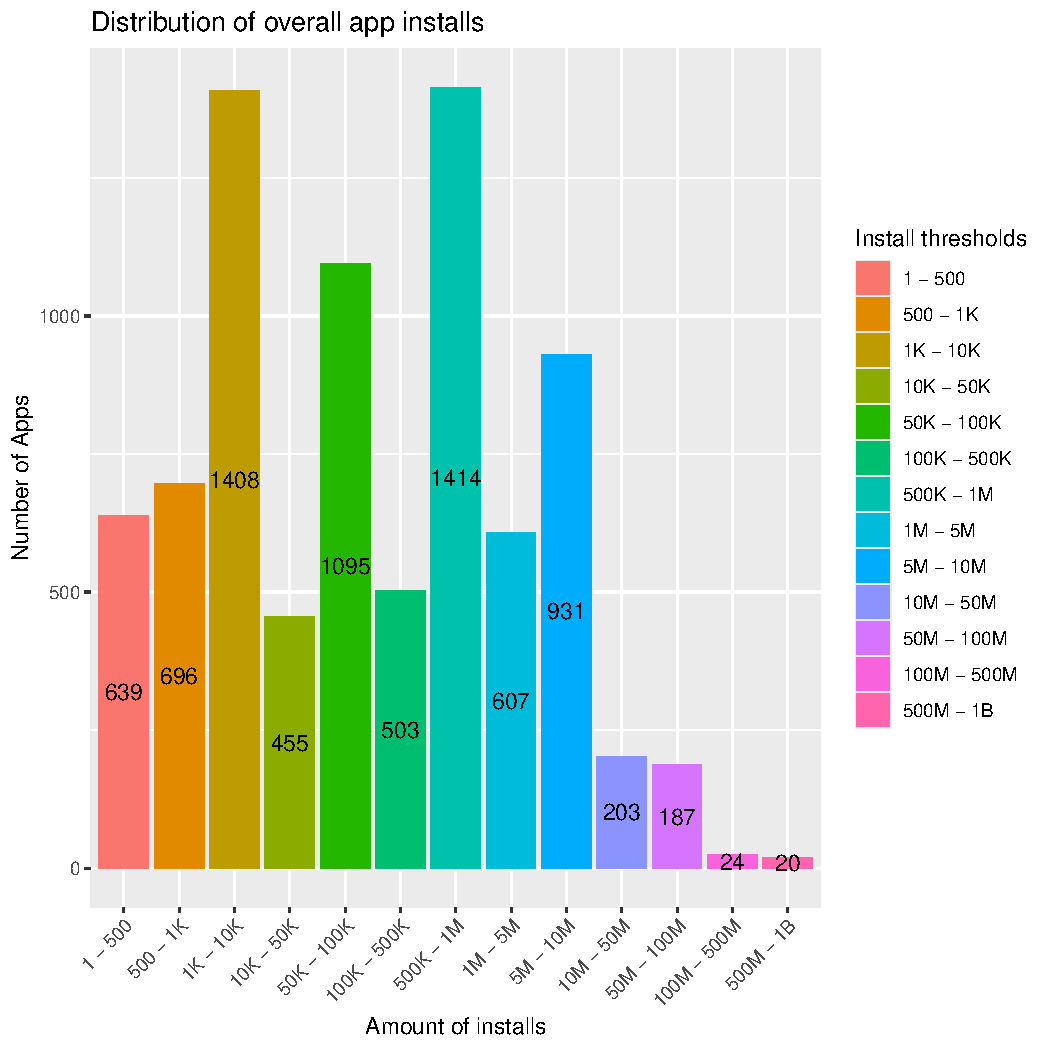
\includegraphics[width=0.75\linewidth]{C:/Users/Lewis/DataspellProjects/DataVis/Assignment/RNW/figures/barOverallInstalls-1} 

}

\caption[Bar chart of install counts]{Bar chart of install counts.}\label{fig:barOverallInstalls}
\end{figure}

\end{knitrout}

We can see that the majority of the dataset contains apps between 1 and 1,000,000 installs. The most common
install threshold for apps to be in is between 1 and 50,000 installs, followed by 500,000 to 1,000,000. This
shows that the market is highly active, and users download a lot of various apps. There are even 20 apps with 
between 500,000,000 and 1,000,000,000 installs, showing how widely used the Play Store is, furthering just how
vital of a market it is to place apps on. 

\begin{knitrout}
\definecolor{shadecolor}{rgb}{0.969, 0.969, 0.969}\color{fgcolor}\begin{kframe}
\begin{alltt}
\hlstd{installCounts} \hlkwb{<-} \hlstd{dataDf} \hlopt
\hlkwd{group_by}\hlstd{(Category)} \hlopt  \hlcom{# Group by the category}
\hlkwd{summarise}\hlstd{(}\hlkwc{count} \hlstd{=} \hlkwd{n}\hlstd{())}   \hlcom{# Count the number of apps in each group}

\hlkwd{ggplot}\hlstd{(installCounts,} \hlkwd{aes}\hlstd{(}\hlkwc{x} \hlstd{= count,} \hlkwc{y} \hlstd{= Category,} \hlkwc{fill} \hlstd{= Category))} \hlopt{+}
\hlkwd{geom_bar}\hlstd{(}\hlkwc{stat} \hlstd{=} \hlstr{"identity"}\hlstd{)} \hlopt{+}
\hlkwd{geom_text}\hlstd{(}\hlkwd{aes}\hlstd{(}\hlkwc{label} \hlstd{= count),}
        \hlcom{# At the end of the bar}
        \hlkwc{position} \hlstd{=} \hlkwd{position_stack}\hlstd{(),} \hlkwc{hjust} \hlstd{=} \hlnum{1}\hlstd{,} \hlkwc{size} \hlstd{=} \hlnum{4}\hlstd{)} \hlopt{+}
\hlkwd{labs}\hlstd{(}\hlkwc{title} \hlstd{=} \hlstr{"Distribution of apps by category"}\hlstd{,}
     \hlkwc{x} \hlstd{=} \hlstr{"Amount of apps"}\hlstd{,} \hlkwc{y} \hlstd{=} \hlstr{"Categories"}\hlstd{)} \hlopt{+}
\hlkwd{theme}\hlstd{(}\hlkwc{axis.text.x} \hlstd{=} \hlkwd{element_text}\hlstd{(}\hlkwc{angle} \hlstd{=}\hlnum{45}\hlstd{,} \hlkwc{hjust} \hlstd{=} \hlnum{1}\hlstd{),}
      \hlkwc{legend.position} \hlstd{=} \hlstr{"none"}\hlstd{)}
\end{alltt}
\end{kframe}\begin{figure}[H]

{\centering 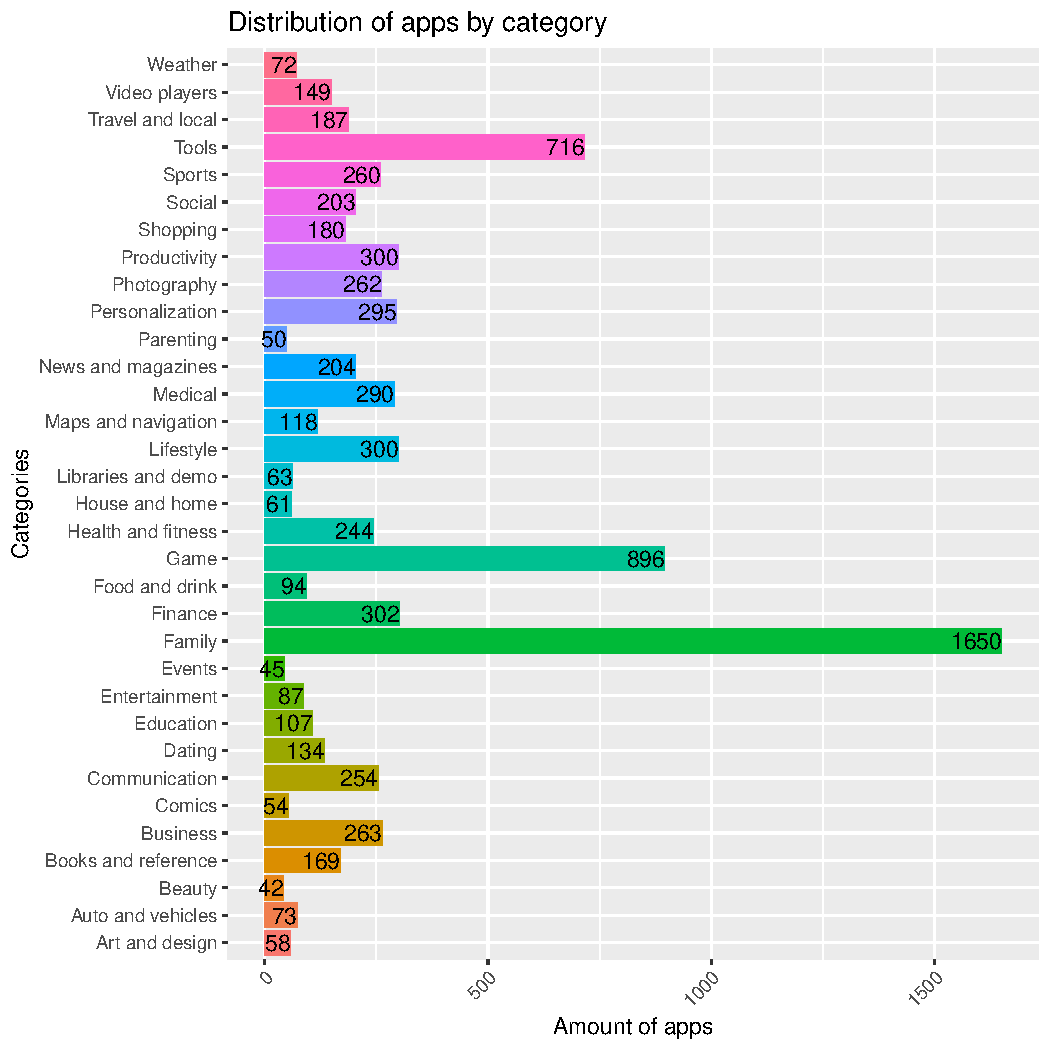
\includegraphics[width=0.75\linewidth]{C:/Users/Lewis/DataspellProjects/DataVis/Assignment/RNW/figures/barCategoryInstalls-1} 

}

\caption[Bar chart of the amount of apps in each category]{Bar chart of the amount of apps in each category.}\label{fig:barCategoryInstalls}
\end{figure}

\end{knitrout}

The market is mostly dominated by apps categorised as "Family" apps, followed by games and tools. This 
suggests that these apps are successful due to the sheer quantity of them in relation to other available
categories, which will be analysed further by checking the ratings of apps by category in Section \ref{sec:answers}

\begin{knitrout}
\definecolor{shadecolor}{rgb}{0.969, 0.969, 0.969}\color{fgcolor}\begin{kframe}
\begin{alltt}
\hlstd{installCounts} \hlkwb{<-} \hlstd{dataDf} \hlopt
\hlkwd{group_by}\hlstd{(numVer)} \hlopt  \hlcom{# Group by the version}
\hlkwd{summarise}\hlstd{(}\hlkwc{count} \hlstd{=} \hlkwd{n}\hlstd{())}   \hlcom{# Count the number of apps in each group}

\hlkwd{ggplot}\hlstd{(installCounts,} \hlkwd{aes}\hlstd{(}\hlkwc{x} \hlstd{= count,} \hlkwc{y} \hlstd{= numVer,} \hlkwc{fill} \hlstd{= numVer))} \hlopt{+}
\hlkwd{geom_bar}\hlstd{(}\hlkwc{stat} \hlstd{=} \hlstr{"identity"}\hlstd{)} \hlopt{+}
\hlkwd{geom_text}\hlstd{(}\hlkwd{aes}\hlstd{(}\hlkwc{label} \hlstd{= count),}
        \hlcom{# Above the bar}
        \hlkwc{position} \hlstd{=} \hlkwd{position_stack}\hlstd{(}\hlkwc{vjust} \hlstd{=} \hlnum{0.75}\hlstd{),} \hlkwc{size} \hlstd{=} \hlnum{4}\hlstd{)} \hlopt{+}
\hlkwd{labs}\hlstd{(}\hlkwc{title} \hlstd{=} \hlstr{"Distribution of apps by minimum Android version"}\hlstd{,}
     \hlkwc{x} \hlstd{=} \hlstr{"Amount of apps"}\hlstd{,} \hlkwc{y} \hlstd{=} \hlstr{"Minimum version required"}\hlstd{)} \hlopt{+}
\hlkwd{theme}\hlstd{(}\hlkwc{axis.text.x} \hlstd{=} \hlkwd{element_text}\hlstd{(}\hlkwc{angle} \hlstd{=}\hlnum{45}\hlstd{,} \hlkwc{hjust} \hlstd{=} \hlnum{1}\hlstd{),}
      \hlkwc{legend.position} \hlstd{=} \hlstr{"none"}\hlstd{)}
\end{alltt}
\end{kframe}\begin{figure}[H]

{\centering 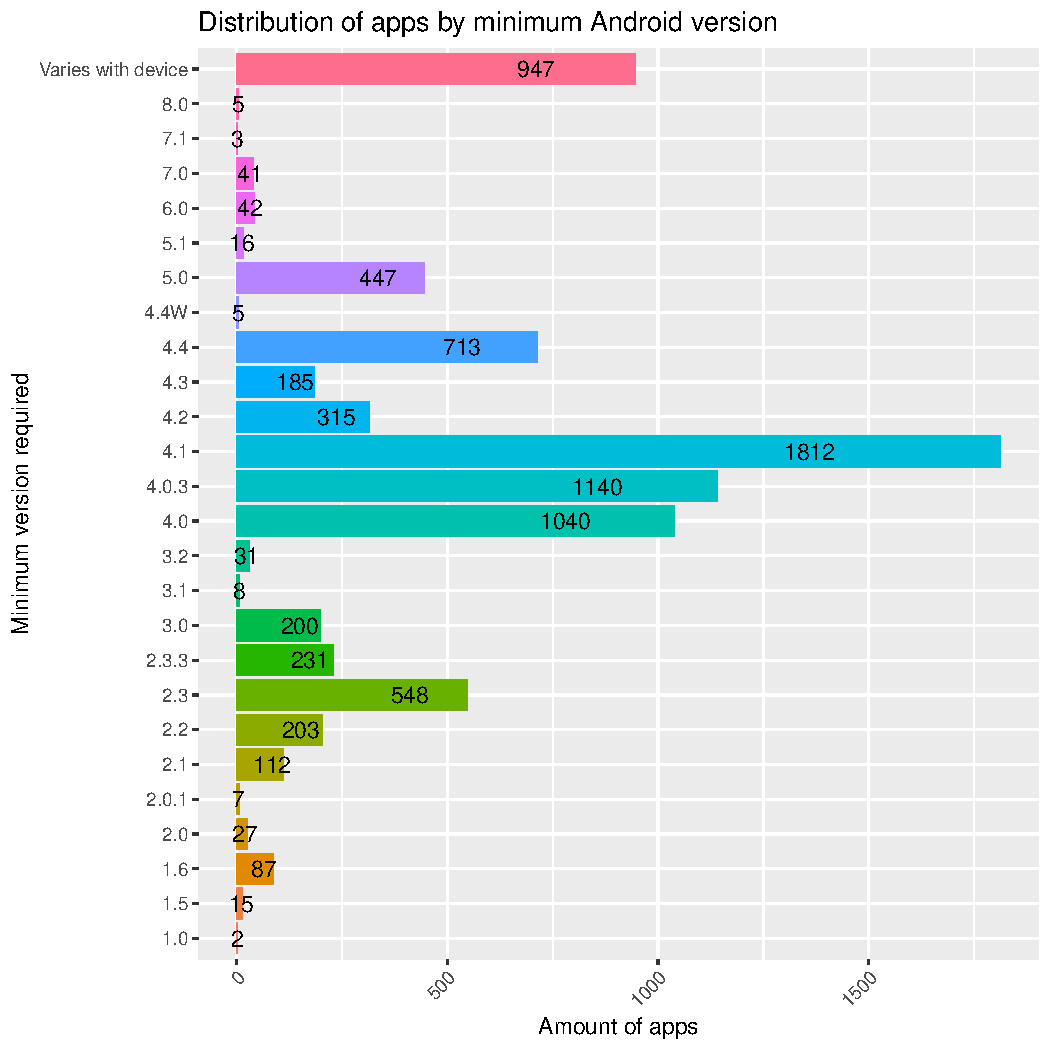
\includegraphics[width=0.75\linewidth]{C:/Users/Lewis/DataspellProjects/DataVis/Assignment/RNW/figures/barAppsVersion-1} 

}

\caption[Bar chart of the amount of apps by minimum required Android version]{Bar chart of the amount of apps by minimum required Android version.}\label{fig:barAppsVersion}
\end{figure}

\end{knitrout}

We can see that a large majority of the apps in the dataset require at least Android version 4.0, which was 
released in 2011. It is ill advised to develop apps below this version, as observed by the trends in Figure
\ref{fig:barAppsVersion} due to their low market share and also how outdated they are, even relative to the time 
of this dataset's publication in 2018.

\begin{knitrout}\footnotesize
\definecolor{shadecolor}{rgb}{0.969, 0.969, 0.969}\color{fgcolor}\begin{kframe}
\begin{alltt}
\hlstd{notVarying} \hlkwb{<-} \hlstd{dataDf} \hlopt
\hlcom{# Have to remove this level because we can't make a string numeric.}
\hlkwd{filter}\hlstd{(numVer} \hlopt{!=} \hlstr{"Varies with device"}\hlstd{)} \hlopt

\hlcom{# Convert values greater than 4 to 4, and values less than 4 to 1.}
\hlcom{# Unfactor comes from the varhandle package, and can return numerics.}
\hlkwd{mutate}\hlstd{(}\hlkwc{numVer} \hlstd{=} \hlkwd{if_else}\hlstd{(}\hlkwd{unfactor}\hlstd{(numVer)} \hlopt{>=} \hlnum{4.0}\hlstd{,} \hlstr{">= 4.0"}\hlstd{,} \hlstr{"< 4.0"}\hlstd{))} \hlopt
\hlkwd{group_by}\hlstd{(numVer)} \hlopt
\hlkwd{summarise}\hlstd{(}\hlkwc{count} \hlstd{=} \hlkwd{n}\hlstd{())}

\hlkwd{ggplot}\hlstd{(notVarying,} \hlkwd{aes}\hlstd{(}\hlkwc{x} \hlstd{=} \hlstr{""}\hlstd{,} \hlkwc{y} \hlstd{= count,} \hlkwc{fill} \hlstd{= numVer,}
                       \hlkwc{label} \hlstd{= scales}\hlopt{::}\hlkwd{percent}\hlstd{(count} \hlopt{/} \hlkwd{sum}\hlstd{(count))))} \hlopt{+}
    \hlkwd{geom_bar}\hlstd{(}\hlkwc{stat} \hlstd{=} \hlstr{"identity"}\hlstd{,} \hlkwc{width} \hlstd{=} \hlnum{1}\hlstd{)} \hlopt{+}
    \hlkwd{geom_text}\hlstd{(}\hlkwc{position} \hlstd{=} \hlkwd{position_stack}\hlstd{(}\hlkwc{vjust} \hlstd{=} \hlnum{0.5}\hlstd{))} \hlopt{+}
    \hlkwd{coord_polar}\hlstd{(}\hlstr{"y"}\hlstd{,} \hlkwc{start} \hlstd{=} \hlnum{0}\hlstd{)} \hlopt{+}
    \hlkwd{labs}\hlstd{(}\hlkwc{title} \hlstd{=} \hlstr{"Minimum required Android versions"}\hlstd{,}
        \hlkwc{fill} \hlstd{=} \hlstr{"Required version"}\hlstd{)} \hlopt{+}
\hlcom{# Change the default blue colours}
    \hlkwd{scale_fill_manual}\hlstd{(}\hlkwc{values}\hlstd{=}\hlkwd{c}\hlstd{(}\hlstr{"#9933FF"}\hlstd{,} \hlstr{"#33FFFF"}\hlstd{),}
                        \hlkwc{labels} \hlstd{=} \hlkwd{c}\hlstd{(}\hlstr{"Less than 4.0"}\hlstd{,} \hlstr{"4.0 or higher"}\hlstd{))} \hlopt{+}
    \hlkwd{theme_void}\hlstd{()} \hlcom{# Hide the axes}
\end{alltt}
\end{kframe}\begin{figure}[H]

{\centering 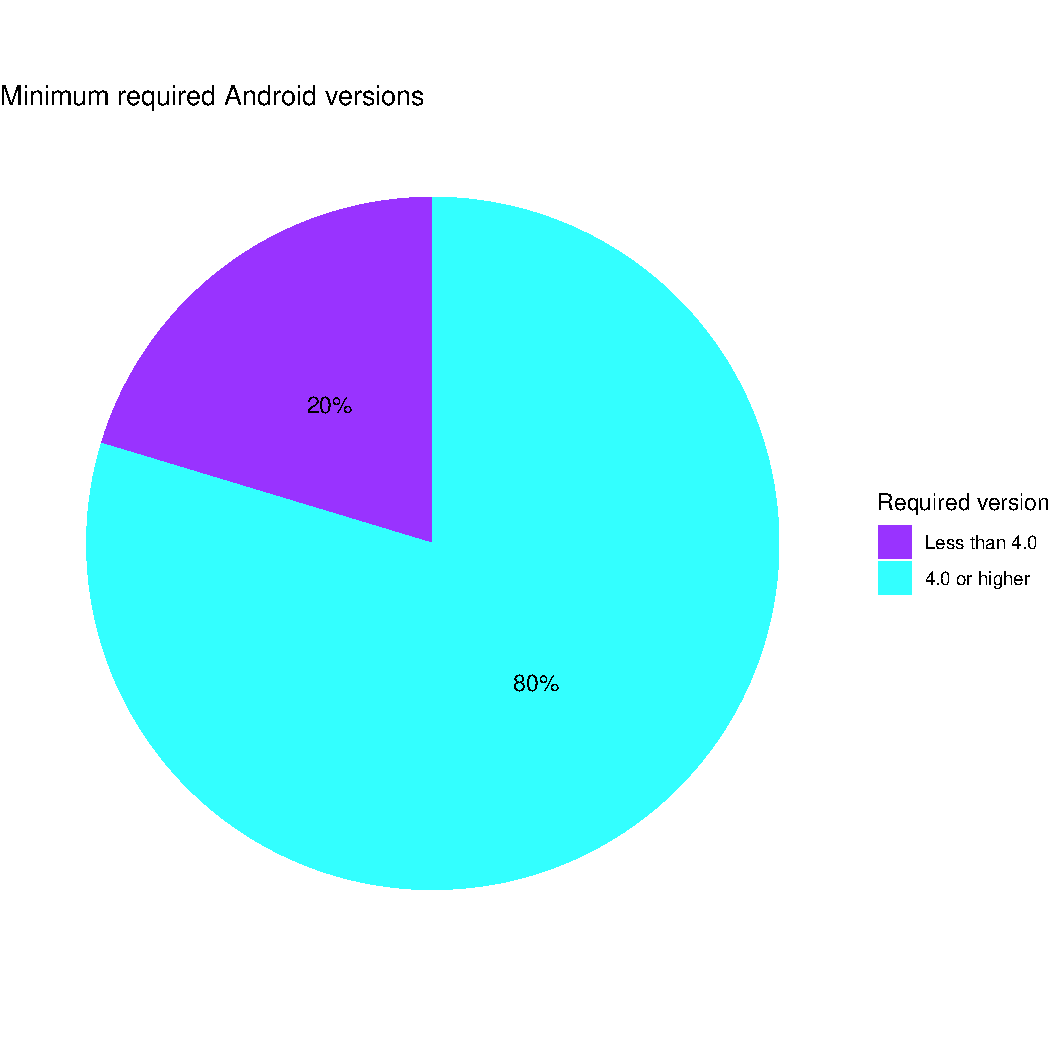
\includegraphics[width=0.75\linewidth]{C:/Users/Lewis/DataspellProjects/DataVis/Assignment/RNW/figures/reqVersion-1} 

}

\caption[Summarisation of required Android versions]{Summarisation of required Android versions}\label{fig:reqVersion}
\end{figure}

\end{knitrout}

\begin{knitrout}
\definecolor{shadecolor}{rgb}{0.969, 0.969, 0.969}\color{fgcolor}\begin{kframe}
\begin{alltt}
\hlkwd{kable}\hlstd{(notVarying,} \hlkwc{caption} \hlstd{=} \hlstr{"Required Android versions"}\hlstd{,} \hlstr{"latex"}\hlstd{)} \hlopt
\hlkwd{kable_styling}\hlstd{(}\hlkwc{latex_options} \hlstd{=} \hlstr{"HOLD_position"}\hlstd{)}
\end{alltt}
\end{kframe}\begin{table}[H]
\centering
\caption{\label{tab:verTbl}Required Android versions}
\centering
\begin{tabular}[t]{l|r}
\hline
numVer & count\\
\hline
< 4.0 & 1471\\
\hline
>= 4.0 & 5764\\
\hline
\end{tabular}
\end{table}

\end{knitrout}

Figure \ref{fig:reqVersion} and Table \ref{tab:verTbl} show how much the market is dominated by apps
of more recent Android versions. Only 20\% of all apps in this dataset have a minimum version below Android 4.0,
likely due to the lack of key features and security maintenance. It is therefore essential to join the remaining
80\% of the market in developing apps for newer Android versions.

\begin{knitrout}
\definecolor{shadecolor}{rgb}{0.969, 0.969, 0.969}\color{fgcolor}\begin{kframe}
\begin{alltt}
\hlstd{pieData} \hlkwb{<-} \hlstd{dataDf} \hlopt
\hlkwd{group_by}\hlstd{(Type)} \hlopt
\hlkwd{summarise}\hlstd{(}\hlkwc{count} \hlstd{=} \hlkwd{n}\hlstd{())}

\hlkwd{ggplot}\hlstd{(pieData,} \hlkwd{aes}\hlstd{(}\hlkwc{x} \hlstd{=} \hlstr{""}\hlstd{,} \hlkwc{y} \hlstd{= count,} \hlkwc{fill} \hlstd{= Type,}
                \hlkwc{label} \hlstd{= scales}\hlopt{::}\hlkwd{percent}\hlstd{(count} \hlopt{/} \hlkwd{sum}\hlstd{(count))))} \hlopt{+}
        \hlkwd{geom_bar}\hlstd{(}\hlkwc{stat} \hlstd{=} \hlstr{"identity"}\hlstd{,} \hlkwc{width} \hlstd{=} \hlnum{1}\hlstd{)} \hlopt{+}
        \hlkwd{geom_text}\hlstd{(}\hlkwc{position} \hlstd{=} \hlkwd{position_stack}\hlstd{(}\hlkwc{vjust} \hlstd{=} \hlnum{0.5}\hlstd{))} \hlopt{+}
        \hlkwd{coord_polar}\hlstd{(}\hlstr{"y"}\hlstd{,} \hlkwc{start} \hlstd{=} \hlnum{0}\hlstd{)} \hlopt{+}
        \hlkwd{labs}\hlstd{(}\hlkwc{title} \hlstd{=} \hlstr{"App type distribution"}\hlstd{,}
            \hlkwc{fill} \hlstd{=} \hlstr{"Type"}\hlstd{)} \hlopt{+}
    \hlcom{# Change the default blue colours to 2 random ones I searched for.}
        \hlkwd{scale_fill_manual}\hlstd{(}\hlkwc{values}\hlstd{=}\hlkwd{c}\hlstd{(}\hlstr{"#A05195"}\hlstd{,} \hlstr{"#FFA600"}\hlstd{),}
                          \hlkwc{labels} \hlstd{=} \hlkwd{c}\hlstd{(}\hlstr{"Free"}\hlstd{,} \hlstr{"Paid"}\hlstd{))} \hlopt{+}
        \hlkwd{theme_void}\hlstd{()} \hlcom{# Hide the axes}
\end{alltt}
\end{kframe}\begin{figure}[H]

{\centering 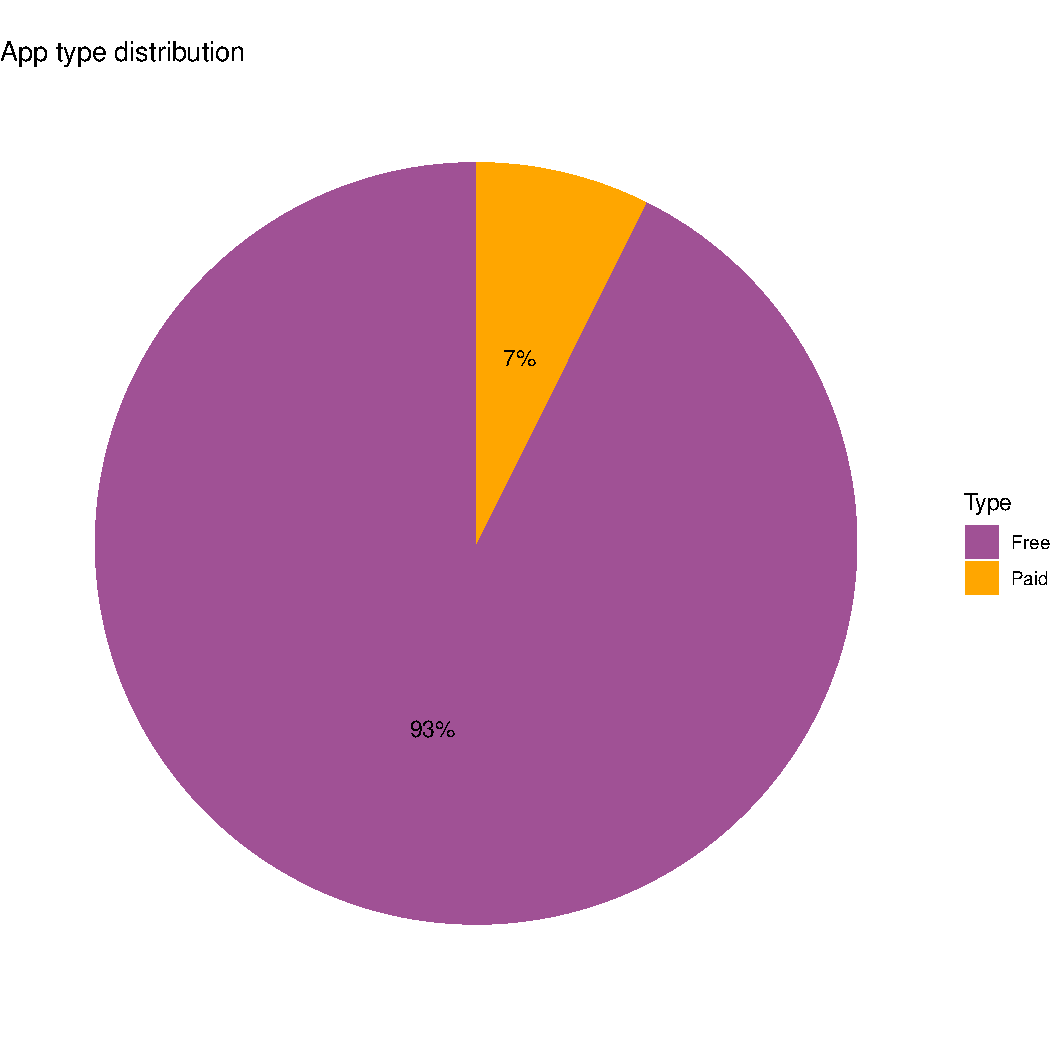
\includegraphics[width=0.75\linewidth]{C:/Users/Lewis/DataspellProjects/DataVis/Assignment/RNW/figures/pieType-1} 

}

\caption[Paid and free app distribution]{Paid and free app distribution}\label{fig:pieType}
\end{figure}

\end{knitrout}

\begin{knitrout}\footnotesize
\definecolor{shadecolor}{rgb}{0.969, 0.969, 0.969}\color{fgcolor}\begin{kframe}
\begin{alltt}
\hlkwd{kable}\hlstd{(pieData,} \hlkwc{caption} \hlstd{=} \hlstr{"Paid and free app distribution"}\hlstd{,} \hlstr{"latex"}\hlstd{)} \hlopt
\hlkwd{kable_styling}\hlstd{(}\hlkwc{latex_options} \hlstd{=} \hlstr{"HOLD_position"}\hlstd{)}
\end{alltt}
\end{kframe}\begin{table}[H]
\centering
\caption{\label{tab:typeTbl}Paid and free app distribution}
\centering
\begin{tabular}[t]{l|r}
\hline
Type & count\\
\hline
Free & 7580\\
\hline
Paid & 602\\
\hline
\end{tabular}
\end{table}

\end{knitrout}

Figure \ref{fig:pieType} and Table \ref{tab:typeTbl} shows us the types of apps in the dataset, meaning 
whether the apps are free to download or whether they cost money. We can see that free apps have a 
93\% market share as opposed to paid apps that account for only 7\%.

\begin{knitrout}
\definecolor{shadecolor}{rgb}{0.969, 0.969, 0.969}\color{fgcolor}\begin{kframe}
\begin{alltt}
\hlstd{doesNotVary} \hlkwb{<-} \hlstd{dataDf} \hlopt
\hlcom{# Grab non-varying sizes by filtering 0.}
\hlkwd{filter}\hlstd{(numSize} \hlopt{!=} \hlstr{"0"}\hlstd{)}

\hlkwd{ggplot}\hlstd{(doesNotVary,} \hlkwd{aes}\hlstd{(}\hlkwc{x} \hlstd{= numSize))} \hlopt{+}
    \hlkwd{geom_histogram}\hlstd{(}\hlkwc{binwidth} \hlstd{=} \hlnum{2}\hlstd{,} \hlkwc{fill} \hlstd{=} \hlstr{"red"}\hlstd{,} \hlkwc{color} \hlstd{=} \hlstr{"black"}\hlstd{)} \hlopt{+}
    \hlkwd{labs}\hlstd{(}\hlkwc{x} \hlstd{=} \hlstr{"App size (in MB)"}\hlstd{,} \hlkwc{y} \hlstd{=} \hlstr{"Number of apps"}\hlstd{,}
         \hlkwc{title} \hlstd{=} \hlstr{"App size distribution"}\hlstd{)} \hlopt{+}
    \hlkwd{theme_minimal}\hlstd{()} \hlopt{+}
    \hlkwd{theme}\hlstd{(}\hlkwc{axis.text.x} \hlstd{=} \hlkwd{element_text}\hlstd{(}\hlkwc{angle} \hlstd{=} \hlnum{45}\hlstd{,} \hlkwc{hjust} \hlstd{=} \hlnum{1}\hlstd{))}
\end{alltt}
\end{kframe}\begin{figure}[H]

{\centering 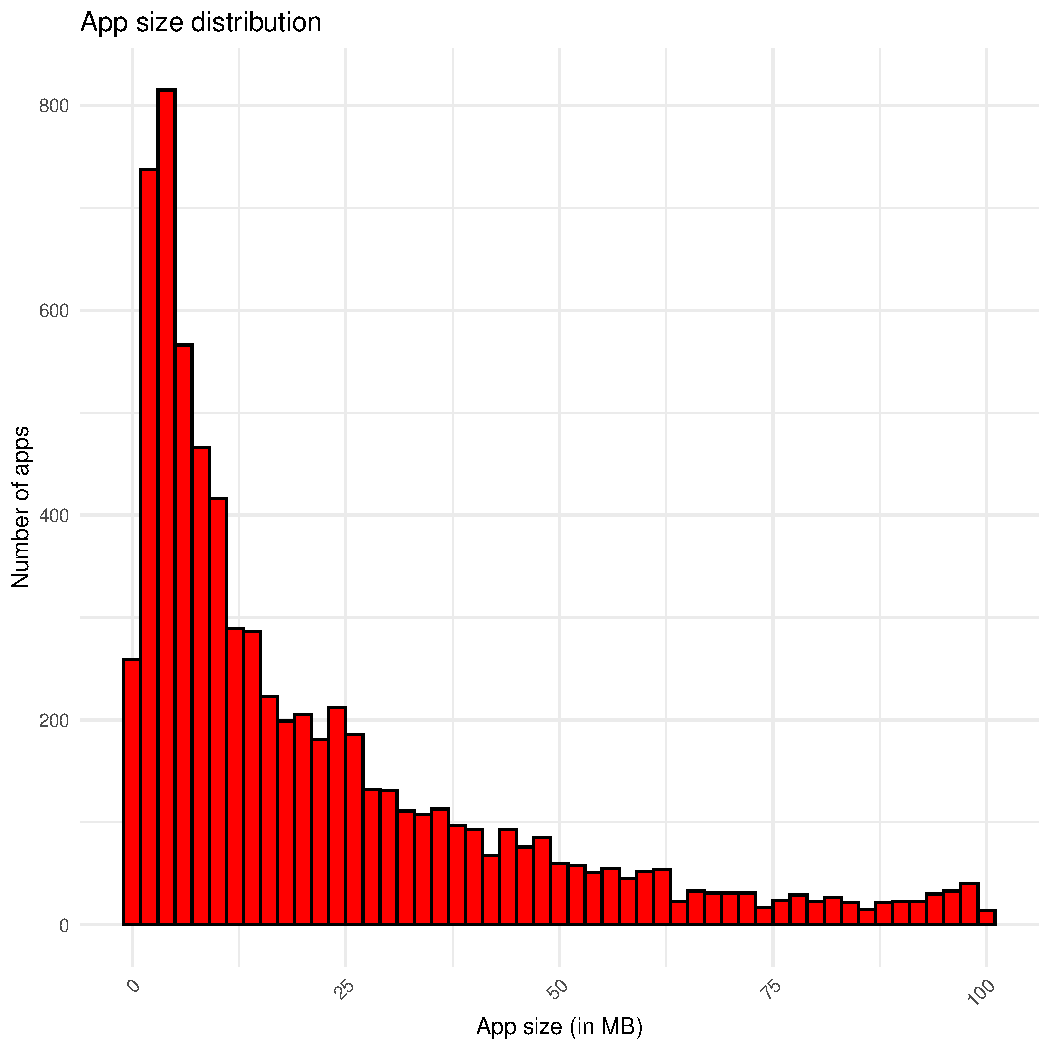
\includegraphics[width=0.75\linewidth]{C:/Users/Lewis/DataspellProjects/DataVis/Assignment/RNW/figures/sizeThresholds-1} 

}

\caption[App size distribution histogram]{App size distribution histogram}\label{fig:sizeThresholds}
\end{figure}

\end{knitrout}

It can be seen that the vast majority of apps in the dataset are all under 20 megabytes in size,
likely due to storage capacities on mobile devices. The correlation between size and install counts
will be analysed in Section \ref{sec:answers}

\begin{knitrout}
\definecolor{shadecolor}{rgb}{0.969, 0.969, 0.969}\color{fgcolor}\begin{kframe}
\begin{alltt}
\hlkwd{ggplot}\hlstd{(dataDf,} \hlkwd{aes}\hlstd{(}\hlkwc{x} \hlstd{=} \hlkwd{month}\hlstd{(Last.Updated,} \hlkwc{label} \hlstd{=} \hlnum{TRUE}\hlstd{)))} \hlopt{+}
    \hlkwd{geom_histogram}\hlstd{(}\hlkwc{fill} \hlstd{=} \hlstr{"skyblue"}\hlstd{,} \hlkwc{color} \hlstd{=} \hlstr{"black"}\hlstd{,}
                   \hlkwc{stat} \hlstd{=} \hlstr{"count"}\hlstd{)} \hlopt{+}
    \hlkwd{labs}\hlstd{(}\hlkwc{x} \hlstd{=} \hlstr{"Date"}\hlstd{,} \hlkwc{y} \hlstd{=} \hlstr{"Frequency"}\hlstd{,}
         \hlkwc{title} \hlstd{=} \hlstr{"Histogram of overall last update dates"}\hlstd{)} \hlopt{+}
    \hlkwd{theme_minimal}\hlstd{()} \hlopt{+}
    \hlkwd{theme}\hlstd{(}\hlkwc{axis.text.x} \hlstd{=} \hlkwd{element_text}\hlstd{(}\hlkwc{angle} \hlstd{=} \hlnum{45}\hlstd{,} \hlkwc{hjust} \hlstd{=} \hlnum{1}\hlstd{))} \hlopt{+}
    \hlkwd{facet_wrap}\hlstd{(}\hlopt{~}\hlkwd{year}\hlstd{(Last.Updated))}
\end{alltt}
\end{kframe}\begin{figure}[H]

{\centering 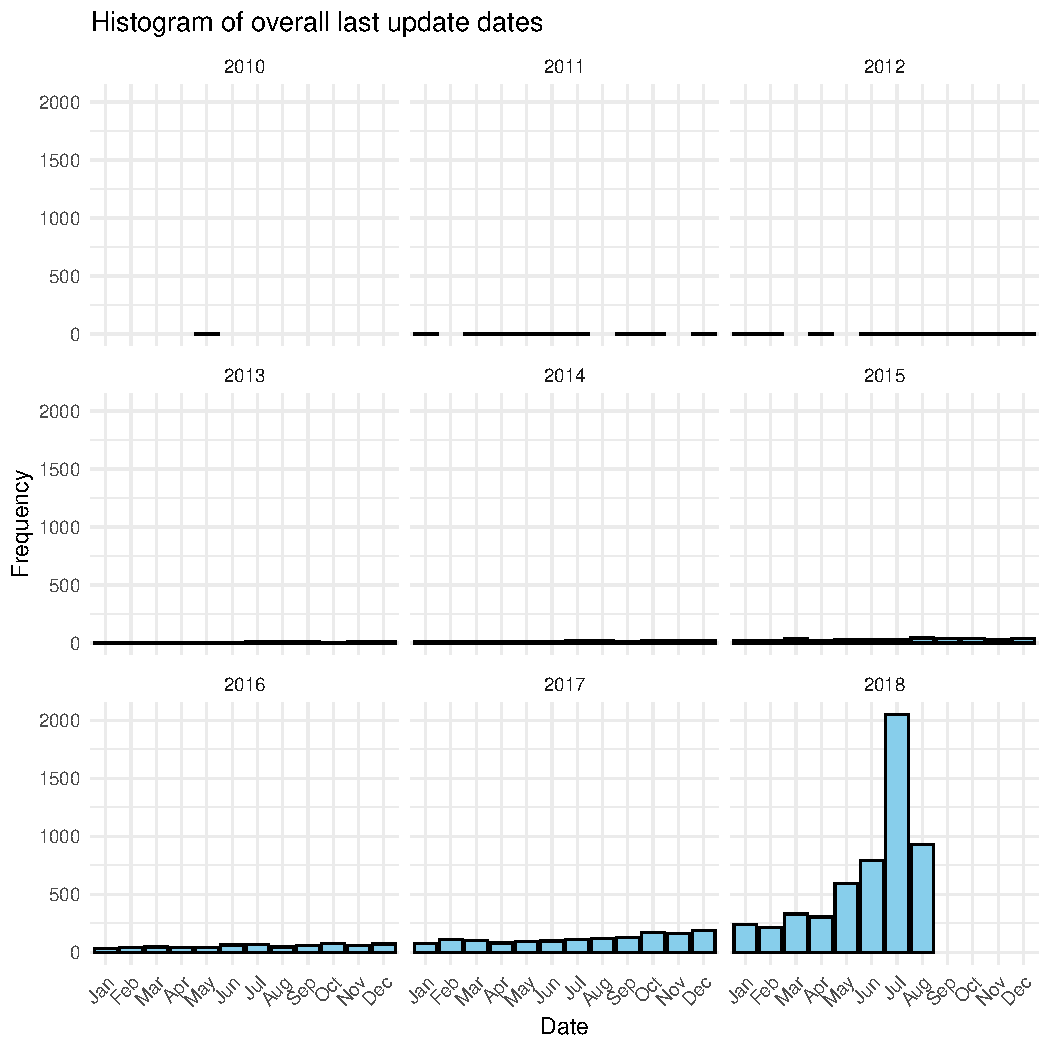
\includegraphics[width=0.75\linewidth]{C:/Users/Lewis/DataspellProjects/DataVis/Assignment/RNW/figures/lastUpdated-1} 

}

\caption[Overall histogram of when apps were last updated]{Overall histogram of when apps were last updated}\label{fig:lastUpdated}
\end{figure}

\end{knitrout}

This histogram reveals that the vast majority of the apps were last updated in 2018, correlating
with the date that this dataset was scraped and released. We can analyse this in further detail by
producing a histogram exclusively of apps that were updated in 2018.

\begin{knitrout}
\definecolor{shadecolor}{rgb}{0.969, 0.969, 0.969}\color{fgcolor}\begin{kframe}
\begin{alltt}
\hlstd{updated2018} \hlkwb{<-} \hlstd{dataDf} \hlopt
\hlkwd{filter}\hlstd{(}\hlkwd{year}\hlstd{(Last.Updated)} \hlopt{==} \hlnum{2018}\hlstd{)}

\hlkwd{ggplot}\hlstd{(updated2018,} \hlkwd{aes}\hlstd{(}\hlkwc{x} \hlstd{= Last.Updated))} \hlopt{+}
    \hlkwd{geom_histogram}\hlstd{(}\hlkwc{binwidth} \hlstd{=} \hlnum{3}\hlstd{,} \hlkwc{fill} \hlstd{=} \hlstr{"orange"}\hlstd{,} \hlkwc{color} \hlstd{=} \hlstr{"black"}\hlstd{)} \hlopt{+}
    \hlkwd{labs}\hlstd{(}\hlkwc{x} \hlstd{=} \hlstr{"Date"}\hlstd{,} \hlkwc{y} \hlstd{=} \hlstr{"Frequency"}\hlstd{,}
         \hlkwc{title} \hlstd{=} \hlstr{"Histogram of updates in 2018"}\hlstd{)} \hlopt{+}
    \hlkwd{theme_minimal}\hlstd{()} \hlopt{+}
    \hlkwd{theme}\hlstd{(}\hlkwc{axis.text.x} \hlstd{=} \hlkwd{element_text}\hlstd{(}\hlkwc{angle} \hlstd{=} \hlnum{45}\hlstd{,} \hlkwc{hjust} \hlstd{=} \hlnum{1}\hlstd{))}
\end{alltt}
\end{kframe}\begin{figure}[H]

{\centering 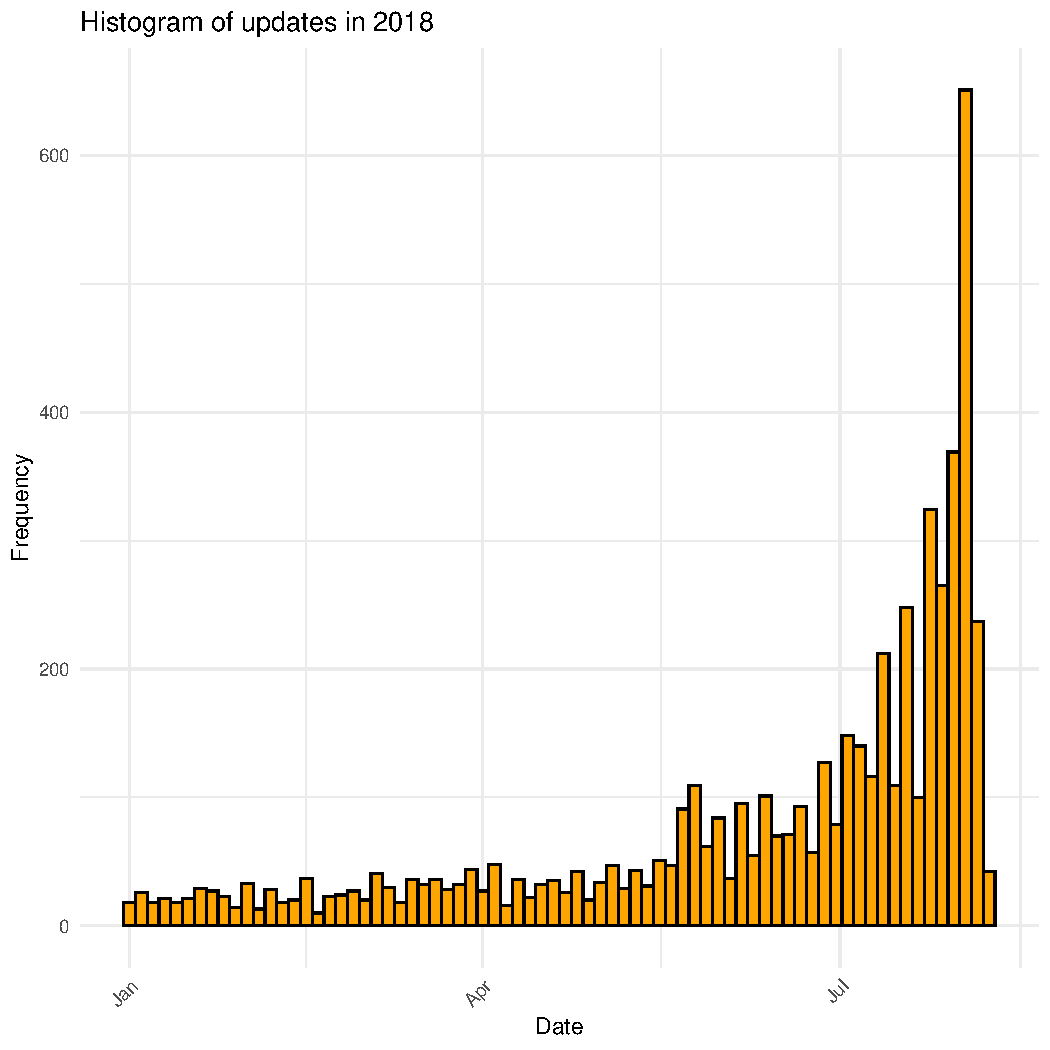
\includegraphics[width=0.75\linewidth]{C:/Users/Lewis/DataspellProjects/DataVis/Assignment/RNW/figures/hist2018apps-1} 

}

\caption[Histogram of app update dates in 2018]{Histogram of app update dates in 2018}\label{fig:hist2018apps}
\end{figure}

\end{knitrout}

We can see from the distribution of Figure \ref{fig:hist2018apps} that the majority of apps 
on the store are updated frequently, as the highest concentration of recent updates is at the time this data was scraped.
This shows the trend that frequent and constant additions of new features or fixing of any bugs is a key element 
in having an app on the Play Store.

\begin{knitrout}
\definecolor{shadecolor}{rgb}{0.969, 0.969, 0.969}\color{fgcolor}\begin{kframe}
\begin{alltt}
\hlstd{updateDays} \hlkwb{<-} \hlstd{dataDf} \hlopt
\hlcom{# label makes the numeric day into the actual day.}
\hlcom{# (0 -> Sunday, 1 -> Monday, etc)}
    \hlkwd{mutate}\hlstd{(}\hlkwc{Day} \hlstd{=} \hlkwd{wday}\hlstd{(Last.Updated,} \hlkwc{label} \hlstd{=} \hlnum{TRUE}\hlstd{))} \hlopt
    \hlkwd{group_by}\hlstd{(Day)} \hlopt
    \hlkwd{summarise}\hlstd{(}\hlkwc{count} \hlstd{=} \hlkwd{n}\hlstd{())}

\hlkwd{ggplot}\hlstd{(updateDays,} \hlkwd{aes}\hlstd{(}\hlkwc{x} \hlstd{=} \hlstr{""}\hlstd{,} \hlkwc{y} \hlstd{= count,} \hlkwc{fill} \hlstd{= Day,}
      \hlkwc{label} \hlstd{= scales}\hlopt{::}\hlkwd{percent}\hlstd{(}\hlkwd{round}\hlstd{(count} \hlopt{/} \hlkwd{sum}\hlstd{(count),} \hlnum{3}\hlstd{))))} \hlopt{+}
    \hlkwd{geom_bar}\hlstd{(}\hlkwc{stat} \hlstd{=} \hlstr{"identity"}\hlstd{,} \hlkwc{width} \hlstd{=} \hlnum{1}\hlstd{)} \hlopt{+}
    \hlkwd{geom_text}\hlstd{(}\hlkwc{position} \hlstd{=} \hlkwd{position_stack}\hlstd{(}\hlkwc{vjust} \hlstd{=} \hlnum{0.5}\hlstd{))} \hlopt{+}
    \hlkwd{coord_polar}\hlstd{(}\hlstr{"y"}\hlstd{,} \hlkwc{start} \hlstd{=} \hlnum{0}\hlstd{)} \hlopt{+}
    \hlkwd{labs}\hlstd{(}\hlkwc{title} \hlstd{=} \hlstr{"Most common days for updates across all years"}\hlstd{)} \hlopt{+}
\hlcom{# Change the default blue colours}
    \hlkwd{scale_fill_brewer}\hlstd{(}\hlkwc{palette} \hlstd{=} \hlstr{"Dark2"}\hlstd{)} \hlopt{+}
    \hlkwd{theme_void}\hlstd{()} \hlcom{# Hide the axes}
\end{alltt}
\end{kframe}\begin{figure}[H]

{\centering 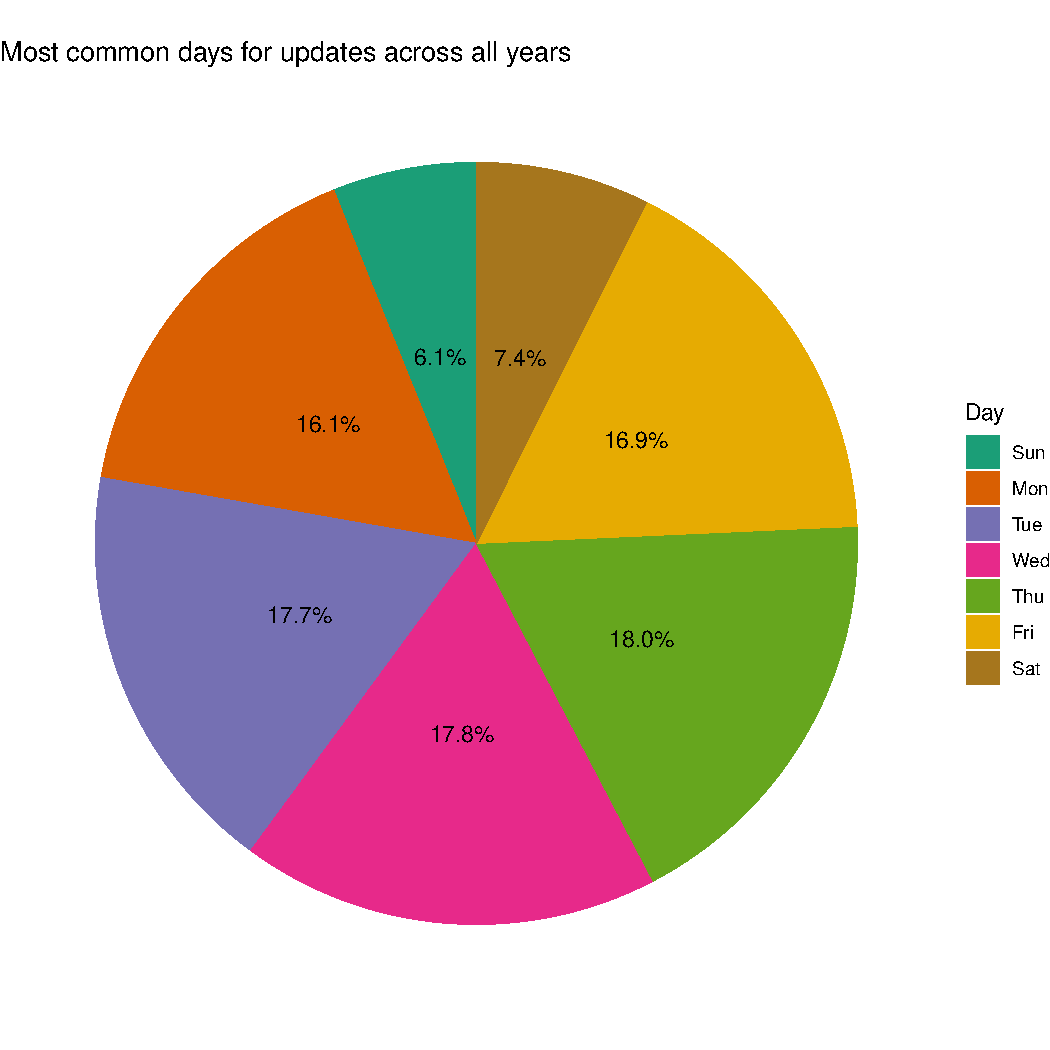
\includegraphics[width=0.75\linewidth]{C:/Users/Lewis/DataspellProjects/DataVis/Assignment/RNW/figures/pieDays-1} 

}

\caption[Days of the week when apps are updated in all documented years]{Days of the week when apps are updated in all documented years}\label{fig:pieDays}
\end{figure}

\end{knitrout}

It can be seen that apps are most commonly updated on weekdays, with Thursday being the most common by a slight
margin. Apps are not commonly updated on weekends, likely due to developers not working these days.


\begin{knitrout}
\definecolor{shadecolor}{rgb}{0.969, 0.969, 0.969}\color{fgcolor}\begin{kframe}
\begin{alltt}
\hlstd{contentRatings} \hlkwb{<-} \hlstd{dataDf} \hlopt
\hlkwd{group_by}\hlstd{(Content.Rating)} \hlopt
\hlkwd{summarise}\hlstd{(}\hlkwc{count} \hlstd{=} \hlkwd{n}\hlstd{())}

\hlkwd{ggplot}\hlstd{(contentRatings,} \hlkwd{aes}\hlstd{(}\hlkwc{x} \hlstd{=} \hlstr{""}\hlstd{,} \hlkwc{y} \hlstd{= count,} \hlkwc{fill} \hlstd{= Content.Rating,}
                       \hlkwc{label} \hlstd{= scales}\hlopt{::}\hlkwd{percent}\hlstd{(count} \hlopt{/} \hlkwd{sum}\hlstd{(count))))} \hlopt{+}
        \hlkwd{geom_bar}\hlstd{(}\hlkwc{stat} \hlstd{=} \hlstr{"identity"}\hlstd{,} \hlkwc{width} \hlstd{=} \hlnum{1}\hlstd{)} \hlopt{+}
        \hlkwd{geom_text}\hlstd{(}\hlkwc{position} \hlstd{=} \hlkwd{position_stack}\hlstd{(}\hlkwc{vjust} \hlstd{=} \hlnum{0.5}\hlstd{))} \hlopt{+}
        \hlkwd{coord_polar}\hlstd{(}\hlstr{"y"}\hlstd{,} \hlkwc{start} \hlstd{=} \hlnum{0}\hlstd{)} \hlopt{+}
        \hlkwd{labs}\hlstd{(}\hlkwc{title} \hlstd{=} \hlstr{"App content rating distribution"}\hlstd{,}
            \hlkwc{fill} \hlstd{=} \hlstr{"Content rating"}\hlstd{)} \hlopt{+}
    \hlcom{# Change the default blue colours}
        \hlkwd{scale_fill_brewer}\hlstd{(}\hlkwc{palette} \hlstd{=} \hlstr{"Pastel1"}\hlstd{)} \hlopt{+}
        \hlkwd{theme_void}\hlstd{()} \hlcom{# Hide the axes}
\end{alltt}
\end{kframe}\begin{figure}[H]

{\centering 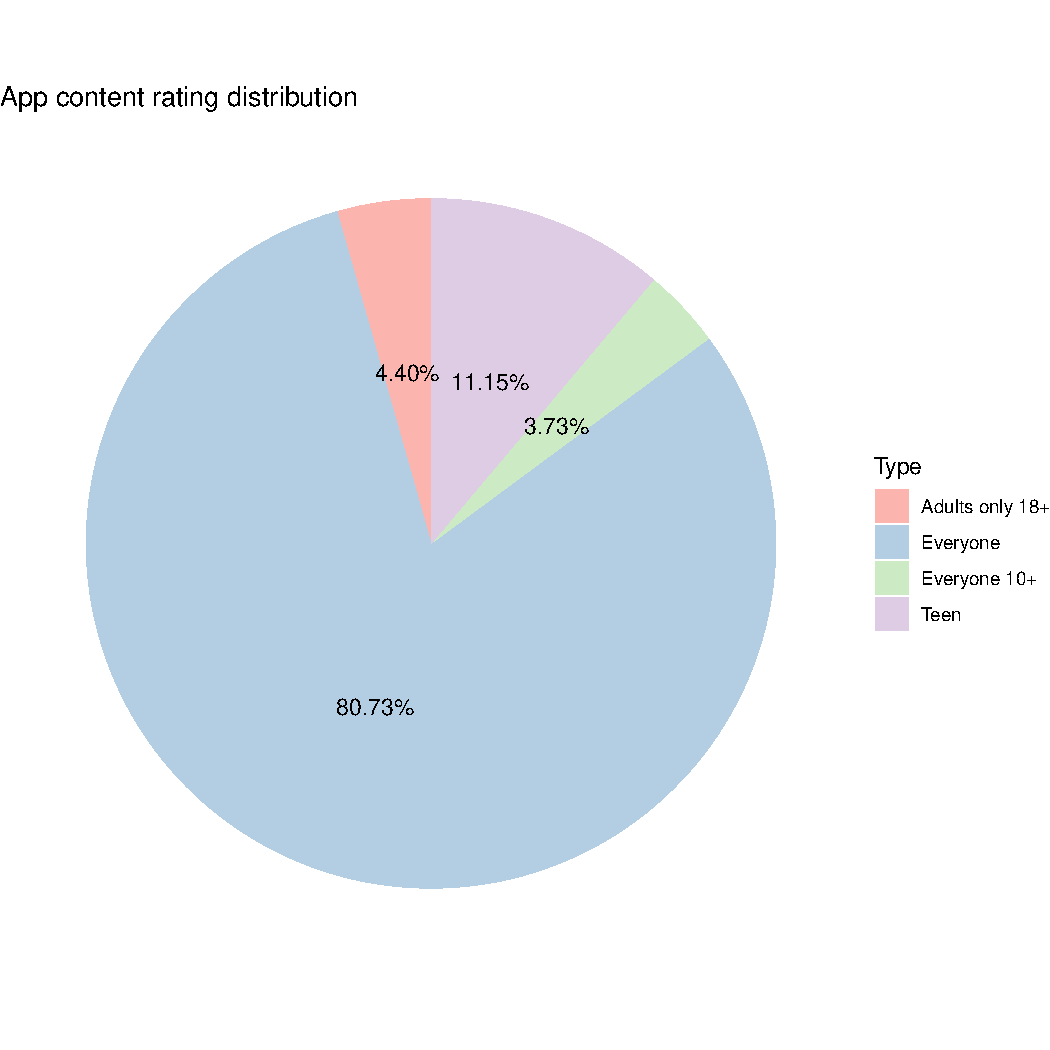
\includegraphics[width=0.75\linewidth]{C:/Users/Lewis/DataspellProjects/DataVis/Assignment/RNW/figures/contentRatingsFrequency-1} 

}

\caption[Distribution of content ratings]{Distribution of content ratings}\label{fig:contentRatingsFrequency}
\end{figure}

\end{knitrout}

Apps targeted at users of all ages are a substantial portion of the dataset showing their high prevalence in 
the market, which is then followed by apps which target teens, apps that target adults only, and apps that
target everyone aged 10 and above.


% Q&A from here
\pagebreak 

\section{Visualisations for question answers}\label{sec:answers}
In this section, the questions posed in Section \ref{sec:questions} will be answered
using the data that has been analysed throughout this report.

\subsection{Is there a correlation between the average review score of an app and its install
count?}

\begin{knitrout}
\definecolor{shadecolor}{rgb}{0.969, 0.969, 0.969}\color{fgcolor}\begin{kframe}
\begin{alltt}
\hlstd{ratingInstalls} \hlkwb{<-} \hlstd{dataDf} \hlopt
\hlkwd{group_by}\hlstd{(installThresholds)} \hlopt
\hlkwd{summarise}\hlstd{(}\hlkwc{avgRating} \hlstd{=} \hlkwd{mean}\hlstd{(Rating))}

\hlkwd{ggplot}\hlstd{(ratingInstalls,} \hlkwd{aes}\hlstd{(}\hlkwc{x} \hlstd{= installThresholds,} \hlkwc{y} \hlstd{= avgRating,}
                           \hlkwc{fill} \hlstd{= installThresholds))} \hlopt{+}
    \hlkwd{geom_bar}\hlstd{(}\hlkwc{stat} \hlstd{=} \hlstr{"identity"}\hlstd{)} \hlopt{+}
    \hlkwd{geom_text}\hlstd{(}\hlkwd{aes}\hlstd{(}\hlkwc{label} \hlstd{=} \hlkwd{round}\hlstd{(avgRating,} \hlnum{3}\hlstd{)),}
              \hlkwc{position} \hlstd{=} \hlkwd{position_stack}\hlstd{(}\hlkwc{vjust} \hlstd{=} \hlnum{0.5}\hlstd{))} \hlopt{+}
    \hlkwd{labs}\hlstd{(}\hlkwc{x} \hlstd{=} \hlstr{"Install Threshold"}\hlstd{,} \hlkwc{y} \hlstd{=} \hlstr{"Average Rating"}\hlstd{,}
         \hlkwc{title} \hlstd{=} \hlstr{"Average Rating by Install Threshold"}\hlstd{)} \hlopt{+}
    \hlkwd{theme}\hlstd{(}\hlkwc{axis.text.x} \hlstd{=} \hlkwd{element_text}\hlstd{(}\hlkwc{angle} \hlstd{=} \hlnum{45}\hlstd{,} \hlkwc{hjust} \hlstd{=} \hlnum{1}\hlstd{),}
          \hlkwc{legend.position} \hlstd{=} \hlstr{"none"}\hlstd{)}
\end{alltt}
\end{kframe}\begin{figure}[H]

{\centering 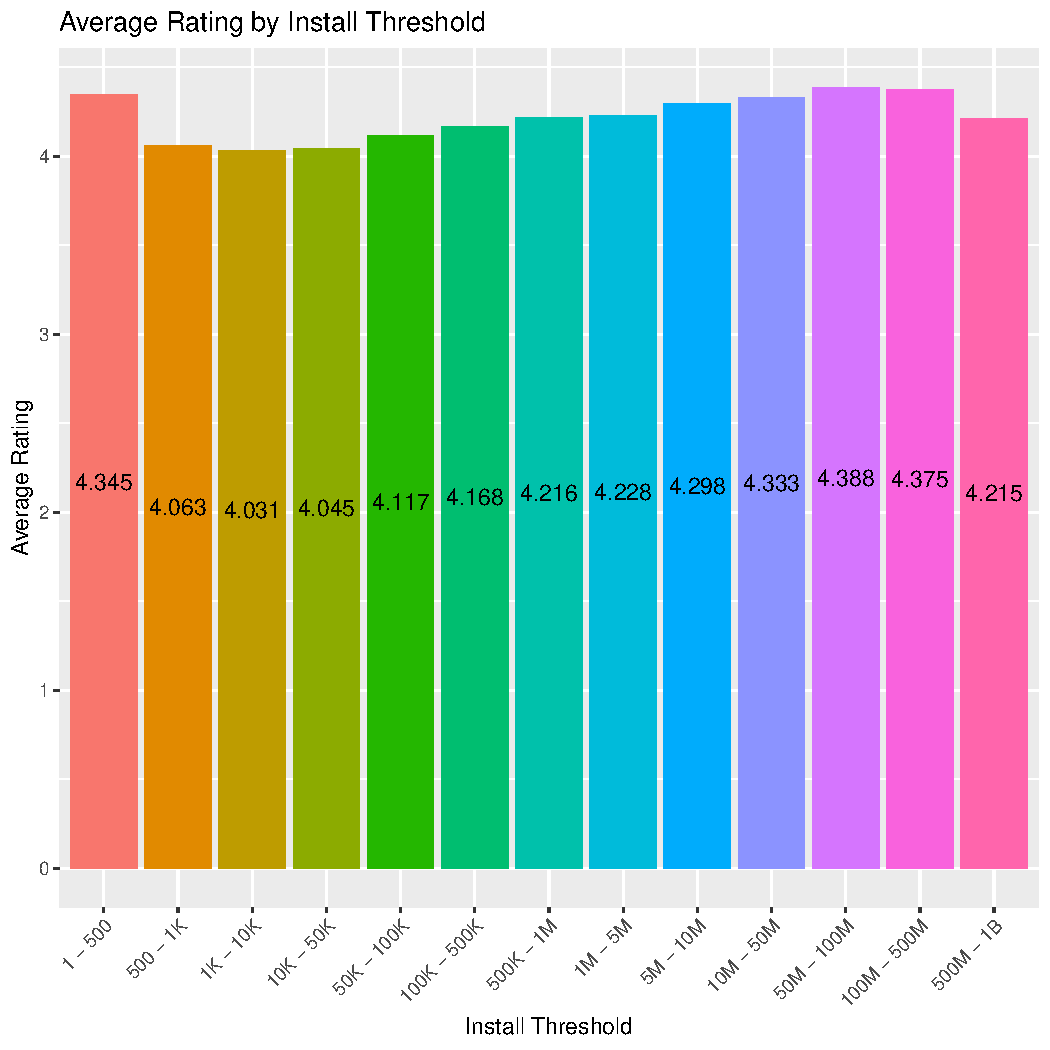
\includegraphics[width=0.75\linewidth]{C:/Users/Lewis/DataspellProjects/DataVis/Assignment/RNW/figures/barRatingsInstalls-1} 

}

\caption[Average rating for apps in each install threshold]{Average rating for apps in each install threshold}\label{fig:barRatingsInstalls}
\end{figure}

\end{knitrout}

From this general bar chart, it can be observed that the average rating across all install thresholds
does not subceed 4. Therefore, this data will be much easier to view in a more zoomed-in format as a line chart,
where a linear regression line can be added to show the trend between installs and rating in closer detail.

\begin{knitrout}
\definecolor{shadecolor}{rgb}{0.969, 0.969, 0.969}\color{fgcolor}\begin{kframe}
\begin{alltt}
\hlkwd{ggplot}\hlstd{(ratingInstalls,} \hlkwd{aes}\hlstd{(}\hlkwc{x} \hlstd{= installThresholds,} \hlkwc{y} \hlstd{= avgRating,}
                           \hlkwc{group} \hlstd{=} \hlnum{1}\hlstd{))} \hlopt{+}
    \hlkwd{geom_point}\hlstd{(}\hlkwd{aes}\hlstd{(}\hlkwc{color} \hlstd{= installThresholds),} \hlkwc{size} \hlstd{=} \hlnum{2}\hlstd{)} \hlopt{+}
    \hlkwd{geom_line}\hlstd{(}\hlkwd{aes}\hlstd{(}\hlkwc{group} \hlstd{=} \hlnum{1}\hlstd{),} \hlkwc{color} \hlstd{=} \hlstr{"skyblue"}\hlstd{)} \hlopt{+}
    \hlkwd{geom_smooth}\hlstd{(}\hlkwc{formula} \hlstd{= y} \hlopt{~} \hlstd{x,} \hlkwc{method} \hlstd{= lm,} \hlkwc{alpha} \hlstd{=} \hlnum{0.1}\hlstd{,}
                \hlkwc{color} \hlstd{=} \hlstr{"orange"}\hlstd{)} \hlopt{+}
    \hlkwd{labs}\hlstd{(}\hlkwc{x} \hlstd{=} \hlstr{"Install Threshold"}\hlstd{,} \hlkwc{y} \hlstd{=} \hlstr{"Average Rating"}\hlstd{,}
         \hlkwc{title} \hlstd{=} \hlstr{"Average Rating by Install Threshold"}\hlstd{)} \hlopt{+}
    \hlkwd{theme}\hlstd{(}\hlkwc{axis.text.x} \hlstd{=} \hlkwd{element_text}\hlstd{(}\hlkwc{angle} \hlstd{=} \hlnum{45}\hlstd{,} \hlkwc{hjust} \hlstd{=} \hlnum{1}\hlstd{),}
          \hlkwc{legend.position} \hlstd{=} \hlstr{"none"}\hlstd{)}
\end{alltt}
\end{kframe}\begin{figure}[H]

{\centering 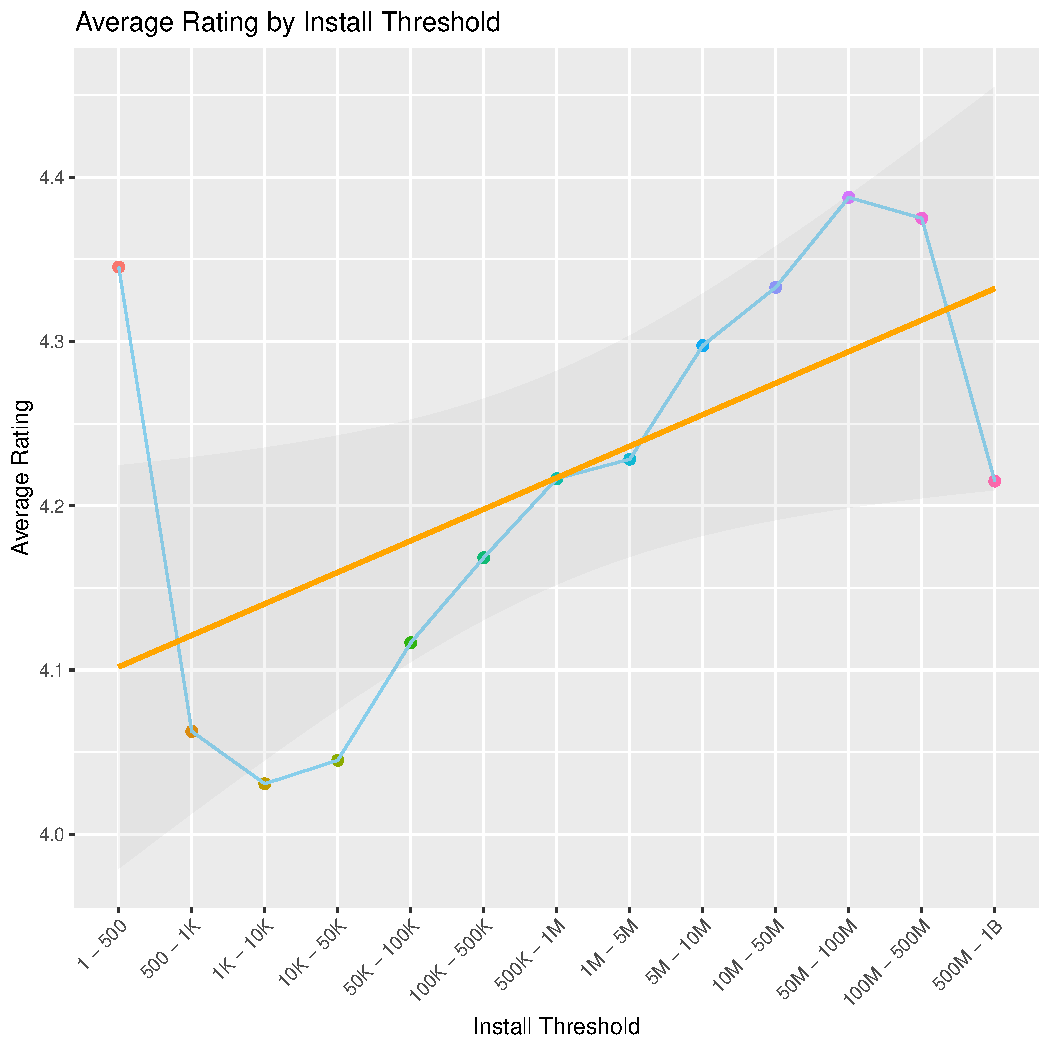
\includegraphics[width=0.75\linewidth]{C:/Users/Lewis/DataspellProjects/DataVis/Assignment/RNW/figures/lineRatingsInstalls-1} 

}

\caption[Zoomed in average rating for apps in each install threshold]{Zoomed in average rating for apps in each install threshold}\label{fig:lineRatingsInstalls}
\end{figure}

\end{knitrout}

From this line graph, the differences in average rating are much clearer. We can observe a mostly positive
correlation between the amount of installs and the average rating of an app. Apps with between 1 and 500 
installs have a very high review score on average due to the low amount of reviews they would have, where 
a single review could skew their overall rating. This is evident immediately with apps between 500
and 50,000 installs suffering from lower average ratings, which likely causes a loop that makes users not
want to install these apps. Past this point, the average rating increases at a mostly linear rate, showing
the strong link between installs and review score. Apps between 500 million and 1 billion reviews have a lower
average review score than the trend would otherwise suggest, which may be due to the specific apps in this 
threshold rather than an overall trend.\\

Overall, this matches the expected answer from Section \ref{sec:questions}.

\pagebreak
\subsection{Which category of app has the highest review score on average?}

\begin{knitrout}
\definecolor{shadecolor}{rgb}{0.969, 0.969, 0.969}\color{fgcolor}\begin{kframe}
\begin{alltt}
\hlstd{filterReviews} \hlkwb{<-} \hlstd{dataDf} \hlopt
    \hlkwd{group_by}\hlstd{(Category)} \hlopt
    \hlkwd{summarise}\hlstd{(}\hlkwc{avgRating} \hlstd{=} \hlkwd{mean}\hlstd{(Rating),} \hlkwc{count} \hlstd{=} \hlkwd{n}\hlstd{())}

\hlkwd{ggplot}\hlstd{(filterReviews,} \hlkwd{aes}\hlstd{(}\hlkwc{x} \hlstd{= avgRating,} \hlkwc{y} \hlstd{= Category,} \hlkwc{fill} \hlstd{= Category))} \hlopt{+}
    \hlkwd{geom_bar}\hlstd{(}\hlkwc{stat} \hlstd{=} \hlstr{"identity"}\hlstd{)} \hlopt{+}
    \hlkwd{geom_text}\hlstd{(}\hlkwd{aes}\hlstd{(}\hlkwc{label} \hlstd{=} \hlkwd{round}\hlstd{(avgRating,} \hlnum{3}\hlstd{)),}
              \hlkwc{position} \hlstd{=} \hlkwd{position_stack}\hlstd{(}\hlkwc{vjust} \hlstd{=} \hlnum{0.5}\hlstd{))} \hlopt{+}
    \hlkwd{labs}\hlstd{(}\hlkwc{title} \hlstd{=} \hlstr{"Average Rating by App Category"}\hlstd{,} \hlkwc{y} \hlstd{=} \hlstr{"App Category"}\hlstd{,}
         \hlkwc{x} \hlstd{=} \hlstr{"Average Rating"}\hlstd{)} \hlopt{+}
    \hlcom{# Too many categories for a legend to reasonably fit.}
    \hlkwd{theme}\hlstd{(}\hlkwc{legend.position} \hlstd{=} \hlstr{"none"}\hlstd{)}
\end{alltt}
\end{kframe}\begin{figure}[H]

{\centering 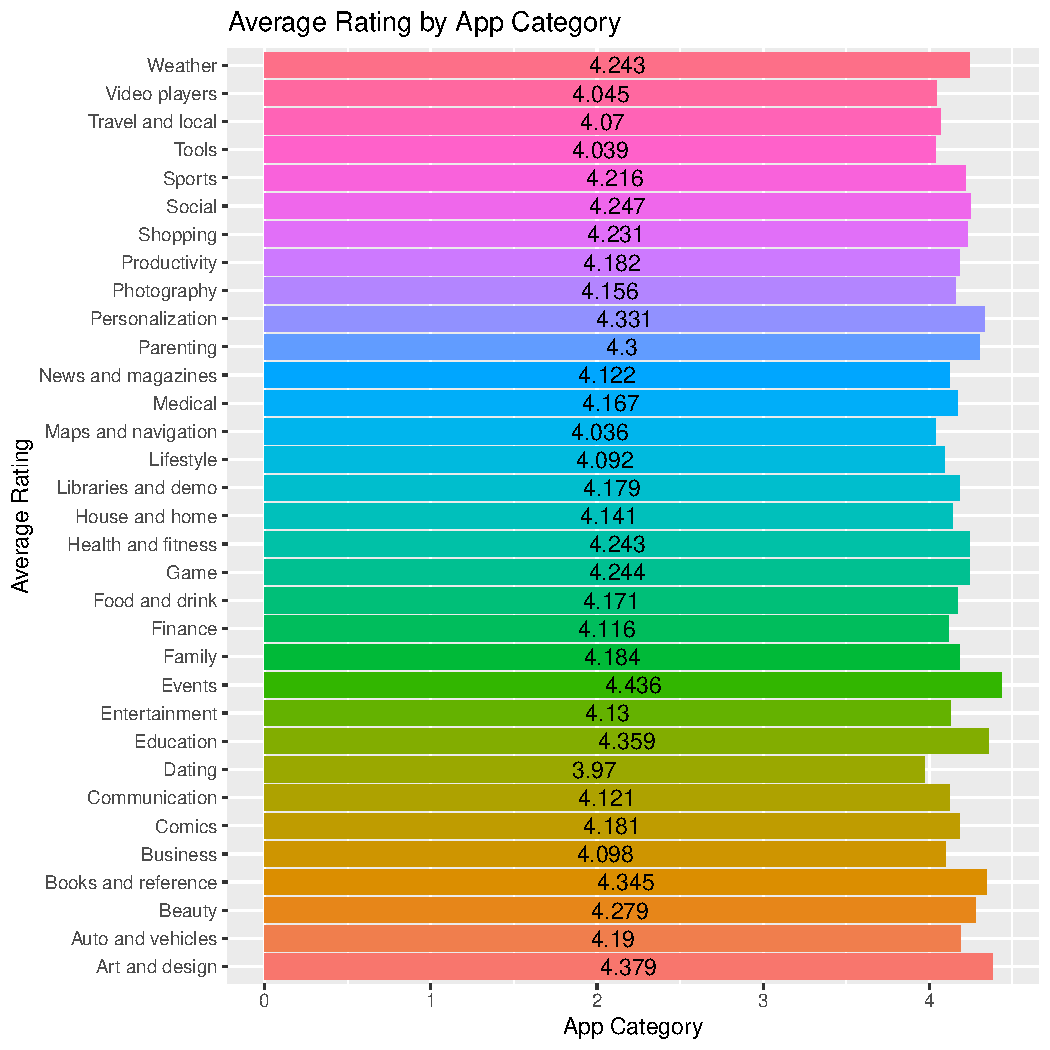
\includegraphics[width=0.75\linewidth]{C:/Users/Lewis/DataspellProjects/DataVis/Assignment/RNW/figures/avgRatingCategory-1} 

}

\caption[Average rating by app category]{Average rating by app category}\label{fig:avgRatingCategory}
\end{figure}

\end{knitrout}

Figure \ref{fig:avgRatingCategory} depicts that the highest rated category is the Events category,
followed by Art and Design and Education. There are 33 categories of app, and the only one to 
have an average rating below 4 is the Dating category, suggesting that developers of this category of app
must prepare for potential lower ratings overall than they would see in other categories. 
In Table \ref{tab:avgRatingTbl} below, the entire data frame used for this graph is shown, with the 
average rating and amount of occurrences of each category in the dataset in descending order.

% Very large table, change to small font.
\footnotesize
\begin{knitrout}
\definecolor{shadecolor}{rgb}{0.969, 0.969, 0.969}\color{fgcolor}\begin{kframe}
\begin{alltt}
\hlcom{# Sort by average rating (descending)}
\hlstd{filterReviews} \hlkwb{<-} \hlkwd{arrange}\hlstd{(filterReviews,} \hlkwd{desc}\hlstd{(avgRating))}

\hlkwd{kable}\hlstd{(filterReviews,} \hlkwc{caption} \hlstd{=} \hlstr{"Categories by review score"}\hlstd{,} \hlstr{"latex"}\hlstd{)} \hlopt
\hlcom{# Large table, so make the font small.}
\hlkwd{kable_styling}\hlstd{(}\hlkwc{font_size} \hlstd{=} \hlnum{8}\hlstd{,} \hlkwc{latex_options} \hlstd{=} \hlkwd{c}\hlstd{(}\hlstr{"HOLD_position"}\hlstd{))}
\end{alltt}
\end{kframe}\begin{table}[H]
\centering
\caption{\label{tab:avgRatingTbl}Categories by review score}
\centering
\fontsize{8}{10}\selectfont
\begin{tabular}[t]{l|r|r}
\hline
Category & avgRating & count\\
\hline
Events & 4.436 & 45\\
\hline
Art and design & 4.379 & 58\\
\hline
Education & 4.359 & 107\\
\hline
Books and reference & 4.345 & 169\\
\hline
Personalization & 4.331 & 295\\
\hline
Parenting & 4.300 & 50\\
\hline
Beauty & 4.279 & 42\\
\hline
Social & 4.247 & 203\\
\hline
Game & 4.244 & 896\\
\hline
Weather & 4.243 & 72\\
\hline
Health and fitness & 4.243 & 244\\
\hline
Shopping & 4.231 & 180\\
\hline
Sports & 4.216 & 260\\
\hline
Auto and vehicles & 4.190 & 73\\
\hline
Family & 4.184 & 1650\\
\hline
Productivity & 4.182 & 300\\
\hline
Comics & 4.181 & 54\\
\hline
Libraries and demo & 4.179 & 63\\
\hline
Food and drink & 4.171 & 94\\
\hline
Medical & 4.167 & 290\\
\hline
Photography & 4.156 & 262\\
\hline
House and home & 4.141 & 61\\
\hline
Entertainment & 4.130 & 87\\
\hline
News and magazines & 4.122 & 204\\
\hline
Communication & 4.121 & 254\\
\hline
Finance & 4.116 & 302\\
\hline
Business & 4.098 & 263\\
\hline
Lifestyle & 4.092 & 300\\
\hline
Travel and local & 4.069 & 187\\
\hline
Video players & 4.045 & 149\\
\hline
Tools & 4.039 & 716\\
\hline
Maps and navigation & 4.036 & 118\\
\hline
Dating & 3.970 & 134\\
\hline
\end{tabular}
\end{table}

\end{knitrout}
% Return to normal size
\normalsize

Table \ref{tab:avgRatingTbl} shows that the most frequent categories (seen in the "count" column) were
the Family, Game and Tools. Of these most frequent categories, Game has the highest average rating, but 
not of the overall categories, meaning the assumption made in Section \ref{sec:questions} was incorrect.

\pagebreak
\subsection{What is the distribution of prices? Are there certain prices used by many apps?}
To properly analyse the distribution of prices, the column will need some modification in order to 
categorise prices and remove apps that do not have a price (free apps) in order to produce readable
visualisations.
\begin{knitrout}\footnotesize
\definecolor{shadecolor}{rgb}{0.969, 0.969, 0.969}\color{fgcolor}\begin{kframe}
\begin{alltt}
\hlcom{# Price has 73 factor levels. }
\hlkwd{nlevels}\hlstd{(dataDf}\hlopt{$}\hlstd{Price)}
\end{alltt}
\begin{verbatim}
[1] 73
\end{verbatim}
\begin{alltt}
\hlcom{# To show the most frequent ones, we can create }
\hlcom{# an ordered list of the most common ones, and consider all the others }
\hlcom{# to be in an "other" category.}

\hlcom{# From the previous graphs, we know that the vast majority (93%) of }
\hlcom{# our dataset is comprised of free apps. Therefore, these will be }
\hlcom{# filtered out to not pollute the graphs with the price point of 0.}
\hlstd{paidApps} \hlkwb{<-} \hlstd{dataDf} \hlopt
\hlkwd{filter}\hlstd{(Price} \hlopt{!=} \hlstr{"0"}\hlstd{)}

\hlkwd{levels}\hlstd{(paidApps}\hlopt{$}\hlstd{Price)}
\end{alltt}
\begin{verbatim}
 [1] "$0.99"   "$1.00"   "$1.20"   "$1.29"   "$1.49"   "$1.50"   "$1.59"  
 [8] "$1.61"   "$1.70"   "$1.75"   "$1.76"   "$1.97"   "$1.99"   "$10.00" 
[15] "$10.99"  "$11.99"  "$12.99"  "$13.99"  "$14.00"  "$14.99"  "$15.46" 
[22] "$15.99"  "$16.99"  "$17.99"  "$18.99"  "$19.40"  "$19.99"  "$2.00"  
[29] "$2.49"   "$2.50"   "$2.56"   "$2.59"   "$2.90"   "$2.95"   "$2.99"  
[36] "$24.99"  "$29.99"  "$299.99" "$3.02"   "$3.04"   "$3.08"   "$3.28"  
[43] "$3.49"   "$3.88"   "$3.90"   "$3.95"   "$3.99"   "$33.99"  "$37.99" 
[50] "$379.99" "$389.99" "$39.99"  "$399.99" "$4.29"   "$4.49"   "$4.59"  
[57] "$4.60"   "$4.77"   "$4.84"   "$4.99"   "$400.00" "$5.49"   "$5.99"  
[64] "$6.49"   "$6.99"   "$7.49"   "$7.99"   "$79.99"  "$8.49"   "$8.99"  
[71] "$9.00"   "$9.99"   "0"      
\end{verbatim}
\begin{alltt}
\hlcom{# Calculate frequency of each price}
\hlstd{priceCounts} \hlkwb{<-} \hlkwd{table}\hlstd{(paidApps}\hlopt{$}\hlstd{Price)}
\hlcom{# Sort the price counts in descending order}
\hlstd{priceCounts} \hlkwb{<-} \hlkwd{sort}\hlstd{(priceCounts,} \hlkwc{decreasing} \hlstd{=} \hlnum{TRUE}\hlstd{)}
\hlcom{# Extract the top 15 levels}
\hlstd{mostCommon} \hlkwb{<-} \hlkwd{names}\hlstd{(priceCounts)[}\hlnum{1}\hlopt{:}\hlnum{15}\hlstd{]}
\hlcom{# Count of other prices combined}
\hlstd{others} \hlkwb{<-} \hlkwd{sum}\hlstd{(priceCounts[}\hlnum{16}\hlopt{:}\hlkwd{length}\hlstd{(priceCounts)])}
\hlcom{# Create a new factor combining top 15 levels and others}
\hlstd{paidApps}\hlopt{$}\hlstd{priceFactor} \hlkwb{<-} \hlkwd{factor}\hlstd{(paidApps}\hlopt{$}\hlstd{Price,} \hlkwc{levels} \hlstd{=} \hlkwd{c}\hlstd{(mostCommon,} \hlstr{"Others"}\hlstd{))}
\hlcom{# Replace levels not in top 15 with "Others"}
\hlstd{paidApps}\hlopt{$}\hlstd{priceFactor[}\hlopt{!}\hlstd{(paidApps}\hlopt{$}\hlstd{priceFactor} \hlopt \hlstd{mostCommon)]} \hlkwb{<-} \hlstr{"Others"}
\hlcom{# Recalculate frequency of each price after combining levels}
\hlstd{priceCounts} \hlkwb{<-} \hlkwd{table}\hlstd{(paidApps}\hlopt{$}\hlstd{priceFactor)}

\hlcom{# Convert to data frame for ggplot}
\hlstd{pricePlot} \hlkwb{<-} \hlkwd{data.frame}\hlstd{(}\hlkwc{Price} \hlstd{=} \hlkwd{names}\hlstd{(priceCounts),}
                        \hlkwc{Frequency} \hlstd{=} \hlkwd{as.numeric}\hlstd{(priceCounts))}
\end{alltt}
\end{kframe}
\end{knitrout}

% Slightly smaller to keep this to one page.
\begin{knitrout}\footnotesize
\definecolor{shadecolor}{rgb}{0.969, 0.969, 0.969}\color{fgcolor}\begin{kframe}
\begin{alltt}
\hlkwd{ggplot}\hlstd{(pricePlot,} \hlkwd{aes}\hlstd{(}\hlkwc{x} \hlstd{= Price,} \hlkwc{y} \hlstd{= Frequency,} \hlkwc{fill} \hlstd{= Price))} \hlopt{+}
    \hlkwd{geom_bar}\hlstd{(}\hlkwc{stat} \hlstd{=} \hlstr{"identity"}\hlstd{)} \hlopt{+}
    \hlkwd{geom_text}\hlstd{(}\hlkwd{aes}\hlstd{(}\hlkwc{label} \hlstd{= Frequency),} \hlkwc{position} \hlstd{=} \hlkwd{position_stack}\hlstd{(}\hlkwc{vjust} \hlstd{=} \hlnum{0.5}\hlstd{))} \hlopt{+}
    \hlkwd{labs}\hlstd{(}\hlkwc{x} \hlstd{=} \hlstr{"Prices"}\hlstd{,} \hlkwc{y} \hlstd{=} \hlstr{"Frequency"}\hlstd{,} \hlkwc{title} \hlstd{=} \hlstr{"App price point frequencies"}\hlstd{)} \hlopt{+}
    \hlcom{# $399.99 and $14.99 would not show in price order normally, so they can }
    \hlcom{# be manually adjusted.}
    \hlkwd{scale_x_discrete}\hlstd{(}\hlkwc{limits} \hlstd{=} \hlkwd{c}\hlstd{(}\hlstr{"$0.99"}\hlstd{,}\hlstr{"$1.49"}\hlstd{,}\hlstr{"$1.99"}\hlstd{,}\hlstr{"$2.49"}\hlstd{,}\hlstr{"$2.99"}\hlstd{,}\hlstr{"$3.49"}\hlstd{,}
                                \hlstr{"$3.99"}\hlstd{,}\hlstr{"$4.49"}\hlstd{,}\hlstr{"$4.99"}\hlstd{,}\hlstr{"$5.99"}\hlstd{,}\hlstr{"$6.99"}\hlstd{,}\hlstr{"$7.99"}\hlstd{,}
                                \hlstr{"$9.99"}\hlstd{,}\hlstr{"$14.99"}\hlstd{,}\hlstr{"$399.99"}\hlstd{,}\hlstr{"Others"}\hlstd{))} \hlopt{+}
    \hlkwd{theme}\hlstd{(}\hlkwc{axis.text.x} \hlstd{=} \hlkwd{element_text}\hlstd{(}\hlkwc{angle} \hlstd{=} \hlnum{45}\hlstd{,} \hlkwc{hjust} \hlstd{=} \hlnum{1}\hlstd{),}
          \hlkwc{legend.position} \hlstd{=} \hlstr{"none"}\hlstd{)}
\end{alltt}
\end{kframe}\begin{figure}[H]

{\centering 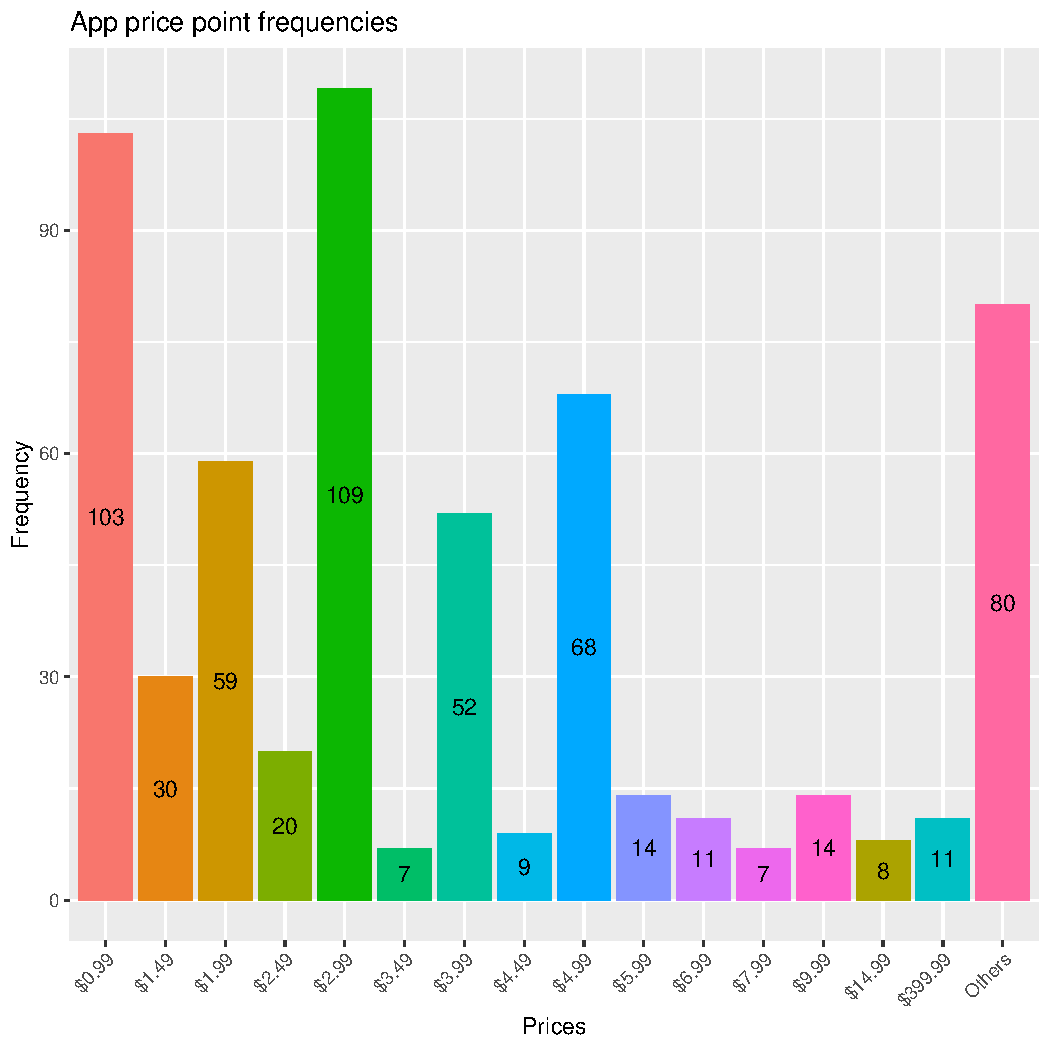
\includegraphics[width=0.75\linewidth]{C:/Users/Lewis/DataspellProjects/DataVis/Assignment/RNW/figures/priceFrequency-1} 

}

\caption[Frequency of app prices]{Frequency of app prices}\label{fig:priceFrequency}
\end{figure}

\end{knitrout}

\begin{knitrout}
\definecolor{shadecolor}{rgb}{0.969, 0.969, 0.969}\color{fgcolor}\begin{kframe}
\begin{alltt}
\hlcom{# Sort by average rating (descending)}
\hlstd{pricePlot} \hlkwb{<-} \hlkwd{arrange}\hlstd{(pricePlot,} \hlkwd{desc}\hlstd{(Frequency))}
\hlcom{# Move "Others" to the bottom of the table.}
\hlstd{pricePlot} \hlkwb{<-} \hlkwd{rbind}\hlstd{(pricePlot[}\hlopt{!}\hlstd{pricePlot}\hlopt{$}\hlstd{Price} \hlopt{==} \hlstr{"Others"}\hlstd{,],}
                   \hlstd{pricePlot[pricePlot}\hlopt{$}\hlstd{Price} \hlopt{==} \hlstr{"Others"}\hlstd{,])}
\hlcom{# Convert back to a tibble to remove the index column.}
\hlstd{pricePlot} \hlkwb{<-} \hlkwd{tibble}\hlstd{(pricePlot)}

\hlcom{# Split over two columns.}
\hlkwd{kable}\hlstd{(}\hlkwd{list}\hlstd{(pricePlot[}\hlnum{1}\hlopt{:}\hlnum{8}\hlstd{,], pricePlot[}\hlnum{9}\hlopt{:}\hlnum{16}\hlstd{,]),} \hlstr{"latex"}\hlstd{)} \hlopt
\hlkwd{kable_styling}\hlstd{(}\hlkwc{latex_options} \hlstd{=} \hlstr{"HOLD_position"}\hlstd{)}
\end{alltt}
\end{kframe}\begin{table}[H]
\centering
\centering
\begin{tabular}[t]{l|r}
\hline
Price & Frequency\\
\hline
\$2.99 & 109\\
\hline
\$0.99 & 103\\
\hline
\$4.99 & 68\\
\hline
\$1.99 & 59\\
\hline
\$3.99 & 52\\
\hline
\$1.49 & 30\\
\hline
\$2.49 & 20\\
\hline
\$5.99 & 14\\
\hline
\end{tabular}
\centering
\begin{tabular}[t]{l|r}
\hline
Price & Frequency\\
\hline
\$9.99 & 14\\
\hline
\$399.99 & 11\\
\hline
\$6.99 & 11\\
\hline
\$4.49 & 9\\
\hline
\$14.99 & 8\\
\hline
\$3.49 & 7\\
\hline
\$7.99 & 7\\
\hline
Others & 80\\
\hline
\end{tabular}
\end{table}

\end{knitrout}

As per Table \ref{tab:typeTbl}, we know that there are only 602 paid apps, which is why Figure \ref{fig:priceFrequency} 
is on a much smaller scale. We can see that 3 of the 5 most common price points for apps are under \$3, meaning
the expectation in \ref{sec:questions} was mostly correct. We can determine that the most common price points used
in the dataset are \$2.99, \$0.99 and \$4.99, suggesting that paid apps should mostly be kept under \$5.
However, this graph yields some additional surprising information,
most notably in the amount of apps that are priced at \$399.99. While it is still a low number at 11, it does still
rank within the top fifteen price points in this dataset. 

\pagebreak
\subsection{Do paid apps receive higher or lower review score on average?}

\begin{knitrout}
\definecolor{shadecolor}{rgb}{0.969, 0.969, 0.969}\color{fgcolor}\begin{kframe}
\begin{alltt}
\hlstd{filterReviews} \hlkwb{<-} \hlstd{dataDf} \hlopt
\hlkwd{group_by}\hlstd{(Type)} \hlopt
    \hlkwd{summarise}\hlstd{(}\hlkwc{avgRating} \hlstd{=} \hlkwd{mean}\hlstd{(Rating),} \hlkwc{count} \hlstd{=} \hlkwd{n}\hlstd{())}

\hlkwd{ggplot}\hlstd{(filterReviews,} \hlkwd{aes}\hlstd{(}\hlkwc{x} \hlstd{= avgRating,} \hlkwc{y} \hlstd{= Type,} \hlkwc{fill} \hlstd{= Type))} \hlopt{+}
    \hlkwd{geom_bar}\hlstd{(}\hlkwc{stat} \hlstd{=} \hlstr{"identity"}\hlstd{)} \hlopt{+}
    \hlkwd{geom_text}\hlstd{(}\hlkwd{aes}\hlstd{(}\hlkwc{label} \hlstd{=} \hlkwd{round}\hlstd{(avgRating,} \hlnum{3}\hlstd{)),}
              \hlkwc{position} \hlstd{=} \hlkwd{position_stack}\hlstd{(}\hlkwc{vjust} \hlstd{=} \hlnum{0.5}\hlstd{))} \hlopt{+}
    \hlkwd{labs}\hlstd{(}\hlkwc{title} \hlstd{=} \hlstr{"Average rating by app type"}\hlstd{,} \hlkwc{x} \hlstd{=} \hlstr{"Average rating"}\hlstd{,}
         \hlkwc{y} \hlstd{=} \hlstr{"App type"}\hlstd{)}
\end{alltt}
\end{kframe}\begin{figure}[H]

{\centering 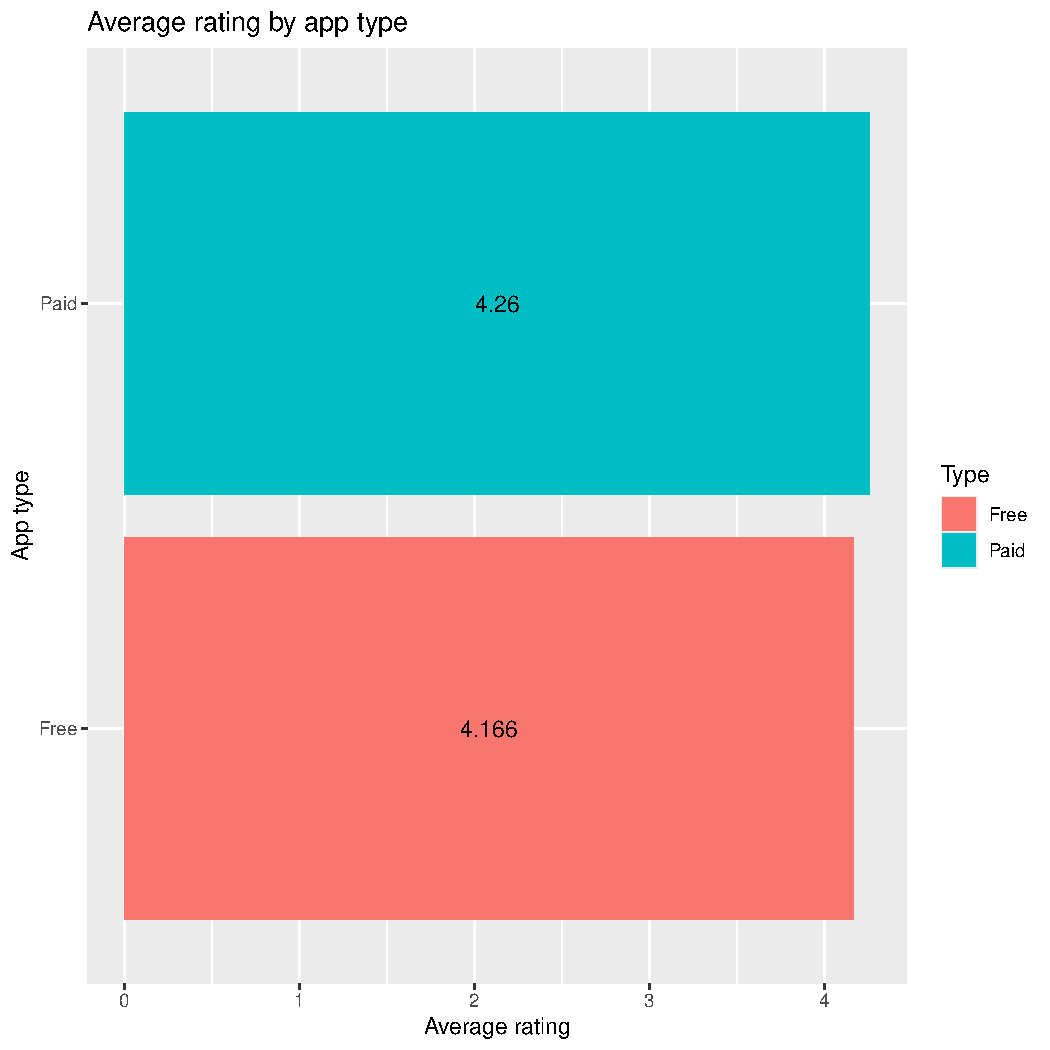
\includegraphics[width=0.75\linewidth]{C:/Users/Lewis/DataspellProjects/DataVis/Assignment/RNW/figures/typeInstalls-1} 

}

\caption[Average rating of paid and free apps]{Average rating of paid and free apps}\label{fig:typeInstalls}
\end{figure}

\end{knitrout}

Surprisingly, Figure \ref{fig:typeInstalls} shows us that paid apps often have a higher 
review score than free apps. This could be due to several factors such as that users who pay for an app might be 
more invested in its success, leading them to be more forgiving of minor issues and more likely to leave a positive 
review. Furthermore, the cost might act as a filter, deterring 
users who wouldn't like the app from downloading it in the first place, leading to a more 
engaged user base with a higher likelihood of leaving positive ratings. 

\pagebreak

\subsection{Is there a correlation between an app's content rating and it's review score?}
Because Figure \ref{fig:contentRatingsFrequency} shows us that a significant portion of the data has 
"Everyone" as its content rating, we can first observe the ratings specifically of that rating, as it would
inflate the Y axis of the visualisations if paired with the others.

\begin{knitrout}
\definecolor{shadecolor}{rgb}{0.969, 0.969, 0.969}\color{fgcolor}\begin{kframe}
\begin{alltt}
\hlstd{everyone} \hlkwb{<-} \hlstd{dataDf} \hlopt
\hlkwd{filter}\hlstd{(Content.Rating} \hlopt{==} \hlstr{"Everyone"}\hlstd{)}

\hlkwd{ggplot}\hlstd{(everyone,} \hlkwd{aes}\hlstd{(}\hlkwc{x} \hlstd{= Rating))} \hlopt{+}
    \hlkwd{geom_histogram}\hlstd{(}\hlkwc{fill} \hlstd{=} \hlstr{"pink"}\hlstd{,} \hlkwc{color} \hlstd{=} \hlstr{"black"}\hlstd{,} \hlkwc{binwidth} \hlstd{=} \hlnum{0.1}\hlstd{)} \hlopt{+}
    \hlkwd{labs}\hlstd{(}\hlkwc{x} \hlstd{=} \hlstr{"Score"}\hlstd{,} \hlkwc{y} \hlstd{=} \hlstr{"Amount of apps"}\hlstd{,}
         \hlkwc{title} \hlstd{=} \hlstr{"Review scores across 'Everyone'"}\hlstd{)} \hlopt{+}
    \hlkwd{theme_minimal}\hlstd{()} \hlopt{+}
    \hlkwd{theme}\hlstd{(}\hlkwc{axis.text.x} \hlstd{=} \hlkwd{element_text}\hlstd{(}\hlkwc{angle} \hlstd{=} \hlnum{45}\hlstd{,} \hlkwc{hjust} \hlstd{=} \hlnum{1}\hlstd{))}
\end{alltt}
\end{kframe}\begin{figure}[H]

{\centering 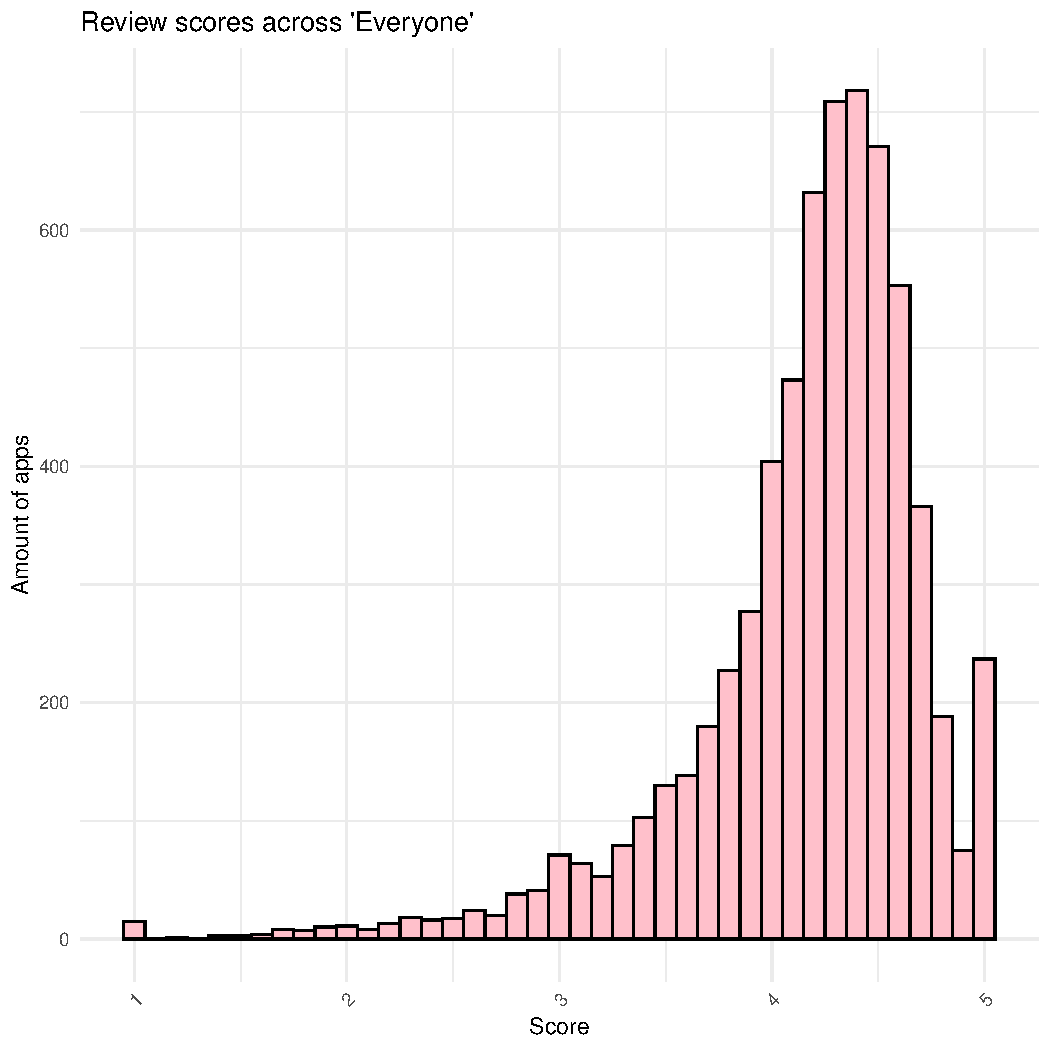
\includegraphics[width=0.75\linewidth]{C:/Users/Lewis/DataspellProjects/DataVis/Assignment/RNW/figures/halfHistContentRatings1-1} 

}

\caption[Review score distributions across the 'Everyone' rating]{Review score distributions across the 'Everyone' rating}\label{fig:halfHistContentRatings1}
\end{figure}

\end{knitrout}

We can see that most apps with the "Everyone" content rating have a review score of over 4,
though there is still a distribution across all scores from 1 to 5. We can see how this compares
against the other content ratings in Figure \ref{fig:halfHistContentRatings2}.

\begin{knitrout}
\definecolor{shadecolor}{rgb}{0.969, 0.969, 0.969}\color{fgcolor}\begin{kframe}
\begin{alltt}
\hlstd{notEveryone} \hlkwb{<-} \hlstd{dataDf} \hlopt
\hlkwd{filter}\hlstd{(Content.Rating} \hlopt{!=} \hlstr{"Everyone"}\hlstd{)}

\hlcom{# binwidth is 0.1 because our ratings are to 1 decimal place.}
\hlkwd{ggplot}\hlstd{(notEveryone,} \hlkwd{aes}\hlstd{(}\hlkwc{x} \hlstd{= Rating))} \hlopt{+}
    \hlkwd{geom_histogram}\hlstd{(}\hlkwc{fill} \hlstd{=} \hlstr{"pink"}\hlstd{,} \hlkwc{color} \hlstd{=} \hlstr{"black"}\hlstd{,} \hlkwc{binwidth} \hlstd{=} \hlnum{0.1}\hlstd{)} \hlopt{+}
    \hlkwd{labs}\hlstd{(}\hlkwc{x} \hlstd{=} \hlstr{"Score"}\hlstd{,} \hlkwc{y} \hlstd{=} \hlstr{"Amount of apps"}\hlstd{,}
         \hlkwc{title} \hlstd{=} \hlstr{"Review scores across all other content ratings"}\hlstd{)} \hlopt{+}
    \hlkwd{theme_minimal}\hlstd{()} \hlopt{+}
    \hlkwd{theme}\hlstd{(}\hlkwc{axis.text.x} \hlstd{=} \hlkwd{element_text}\hlstd{(}\hlkwc{angle} \hlstd{=} \hlnum{45}\hlstd{,} \hlkwc{hjust} \hlstd{=} \hlnum{1}\hlstd{))} \hlopt{+}
    \hlkwd{facet_wrap}\hlstd{(}\hlopt{~}\hlstd{Content.Rating,} \hlkwc{ncol} \hlstd{=} \hlnum{3}\hlstd{)}
\end{alltt}
\end{kframe}\begin{figure}[H]

{\centering 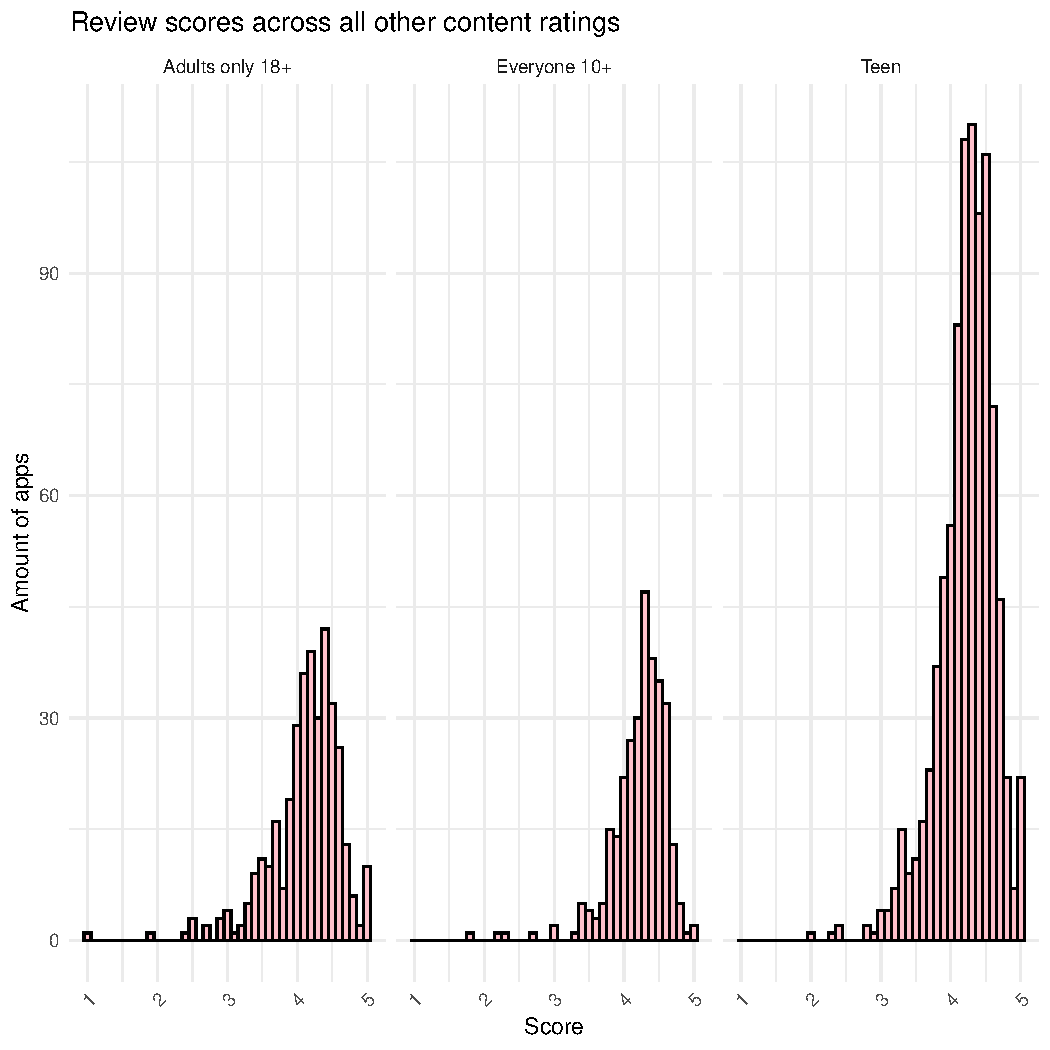
\includegraphics[width=0.75\linewidth]{C:/Users/Lewis/DataspellProjects/DataVis/Assignment/RNW/figures/halfHistContentRatings2-1} 

}

\caption[Review score distributions across other content ratings]{Review score distributions across other content ratings}\label{fig:halfHistContentRatings2}
\end{figure}

\end{knitrout}

We can see that this pattern mostly repeats across all content ratings, though it can also be observed
that apps with a content rating of "Adults only 18+" have a higher concentration of reviews lower than 4.
This can be analysed further with a bar chart as shown in Figure \ref{fig:barContentRatings}.


\begin{knitrout}\footnotesize
\definecolor{shadecolor}{rgb}{0.969, 0.969, 0.969}\color{fgcolor}\begin{kframe}
\begin{alltt}
\hlstd{ratingInstalls} \hlkwb{<-} \hlstd{dataDf} \hlopt
    \hlkwd{group_by}\hlstd{(Content.Rating)} \hlopt
    \hlkwd{summarise}\hlstd{(}\hlkwc{avgRating} \hlstd{=} \hlkwd{mean}\hlstd{(Rating))}

\hlkwd{ggplot}\hlstd{(ratingInstalls,} \hlkwd{aes}\hlstd{(}\hlkwc{x} \hlstd{= Content.Rating,} \hlkwc{y} \hlstd{= avgRating,}
                           \hlkwc{fill} \hlstd{= Content.Rating))} \hlopt{+}
    \hlkwd{geom_bar}\hlstd{(}\hlkwc{stat} \hlstd{=} \hlstr{"identity"}\hlstd{)} \hlopt{+}
    \hlkwd{geom_text}\hlstd{(}\hlkwd{aes}\hlstd{(}\hlkwc{label} \hlstd{=} \hlkwd{round}\hlstd{(avgRating,} \hlnum{3}\hlstd{)),}
              \hlkwc{position} \hlstd{=} \hlkwd{position_stack}\hlstd{(}\hlkwc{vjust} \hlstd{=} \hlnum{0.5}\hlstd{))} \hlopt{+}
    \hlkwd{labs}\hlstd{(}\hlkwc{x} \hlstd{=} \hlstr{"Content age rating"}\hlstd{,} \hlkwc{y} \hlstd{=} \hlstr{"Average review score"}\hlstd{,}
         \hlkwc{title} \hlstd{=} \hlstr{"Average review score by content age rating"}\hlstd{)} \hlopt{+}
    \hlkwd{theme}\hlstd{(}\hlkwc{axis.text.x} \hlstd{=} \hlkwd{element_text}\hlstd{(}\hlkwc{angle} \hlstd{=} \hlnum{45}\hlstd{,} \hlkwc{hjust} \hlstd{=} \hlnum{1}\hlstd{),}
          \hlkwc{legend.position} \hlstd{=} \hlstr{"none"}\hlstd{)}
\end{alltt}
\end{kframe}\begin{figure}[H]

{\centering 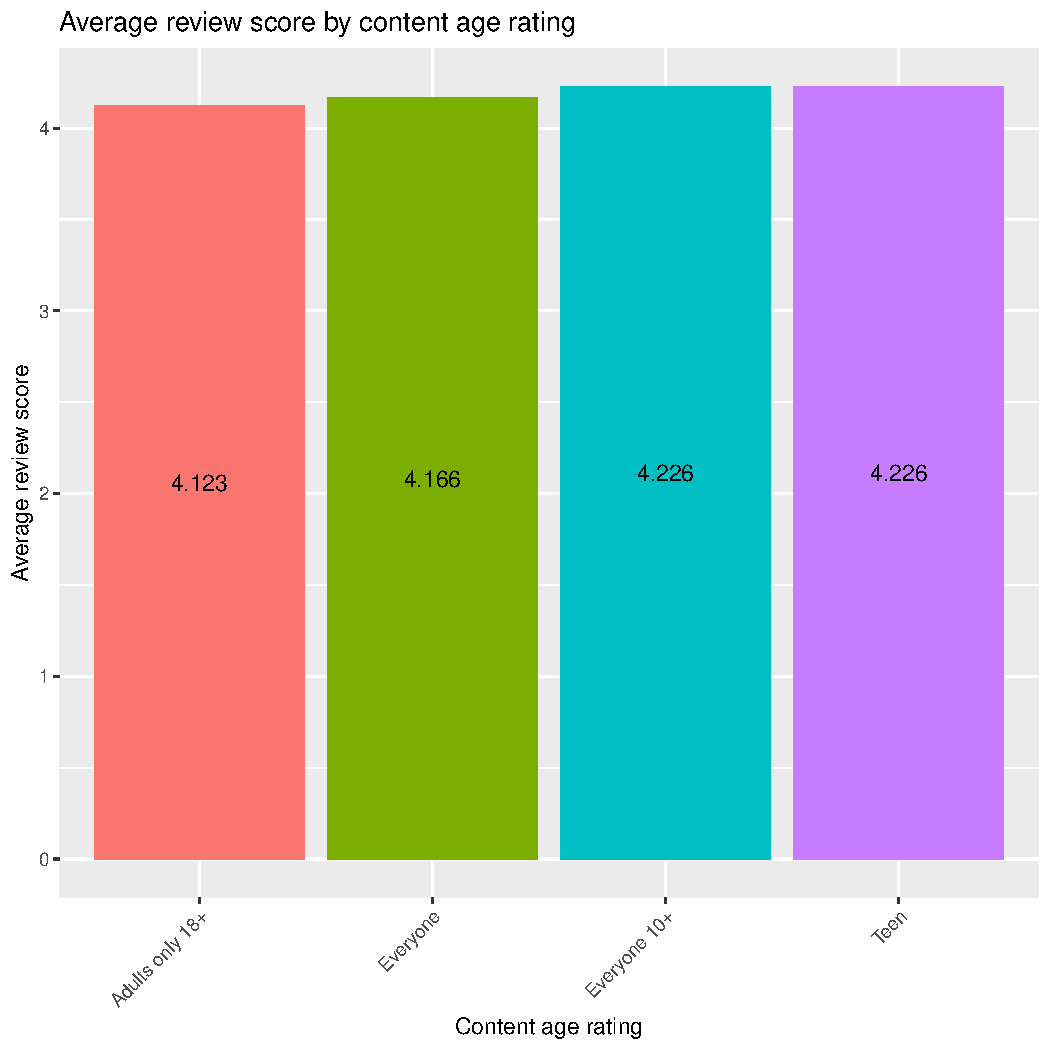
\includegraphics[width=0.75\linewidth]{C:/Users/Lewis/DataspellProjects/DataVis/Assignment/RNW/figures/barContentRatings-1} 

}

\caption[Average review score for each content rating]{Average review score for each content rating}\label{fig:barContentRatings}
\end{figure}

\end{knitrout}

"Adults only" is indeed the lowest rated category. This subverts the expectation
stated in Section \ref{sec:questions}. This is likely due to the trends in Figure \ref{fig:avgRatingCategory} where Dating
apps were rated lower than all others. Dating apps are all 18+ by nature, so they would bring down
the average of their associated content rating. 


\pagebreak
\subsection{Does app size play a role in install count?}

\begin{knitrout}
\definecolor{shadecolor}{rgb}{0.969, 0.969, 0.969}\color{fgcolor}\begin{kframe}
\begin{alltt}
\hlcom{# Filter out apps that vary in size.}
\hlcom{# Because "Varies with device" was changed to 0 earlier, remove 0.}
\hlstd{installsSize} \hlkwb{<-} \hlstd{dataDf} \hlopt
\hlkwd{filter}\hlstd{(numSize} \hlopt{!=} \hlnum{0}\hlstd{)} \hlopt
\hlkwd{group_by}\hlstd{(installThresholds, numSize)}

\hlkwd{ggplot}\hlstd{(installsSize,} \hlkwd{aes}\hlstd{(}\hlkwc{x}\hlstd{=installThresholds,} \hlkwc{y}\hlstd{=numSize))} \hlopt{+}
    \hlkwd{geom_boxplot}\hlstd{(}\hlkwc{fill}\hlstd{=}\hlstr{'skyblue'}\hlstd{)} \hlopt{+}
    \hlkwd{labs}\hlstd{(}\hlkwc{title} \hlstd{=} \hlstr{"App installs by size"}\hlstd{,} \hlkwc{x} \hlstd{=} \hlstr{"Installs"}\hlstd{,}
         \hlkwc{y} \hlstd{=} \hlstr{"Size in MB"}\hlstd{)} \hlopt{+}
    \hlkwd{theme}\hlstd{(}\hlkwc{axis.text.x} \hlstd{=} \hlkwd{element_text}\hlstd{(}\hlkwc{angle} \hlstd{=} \hlnum{45}\hlstd{,} \hlkwc{hjust} \hlstd{=} \hlnum{1}\hlstd{))}
\end{alltt}
\end{kframe}\begin{figure}[H]

{\centering 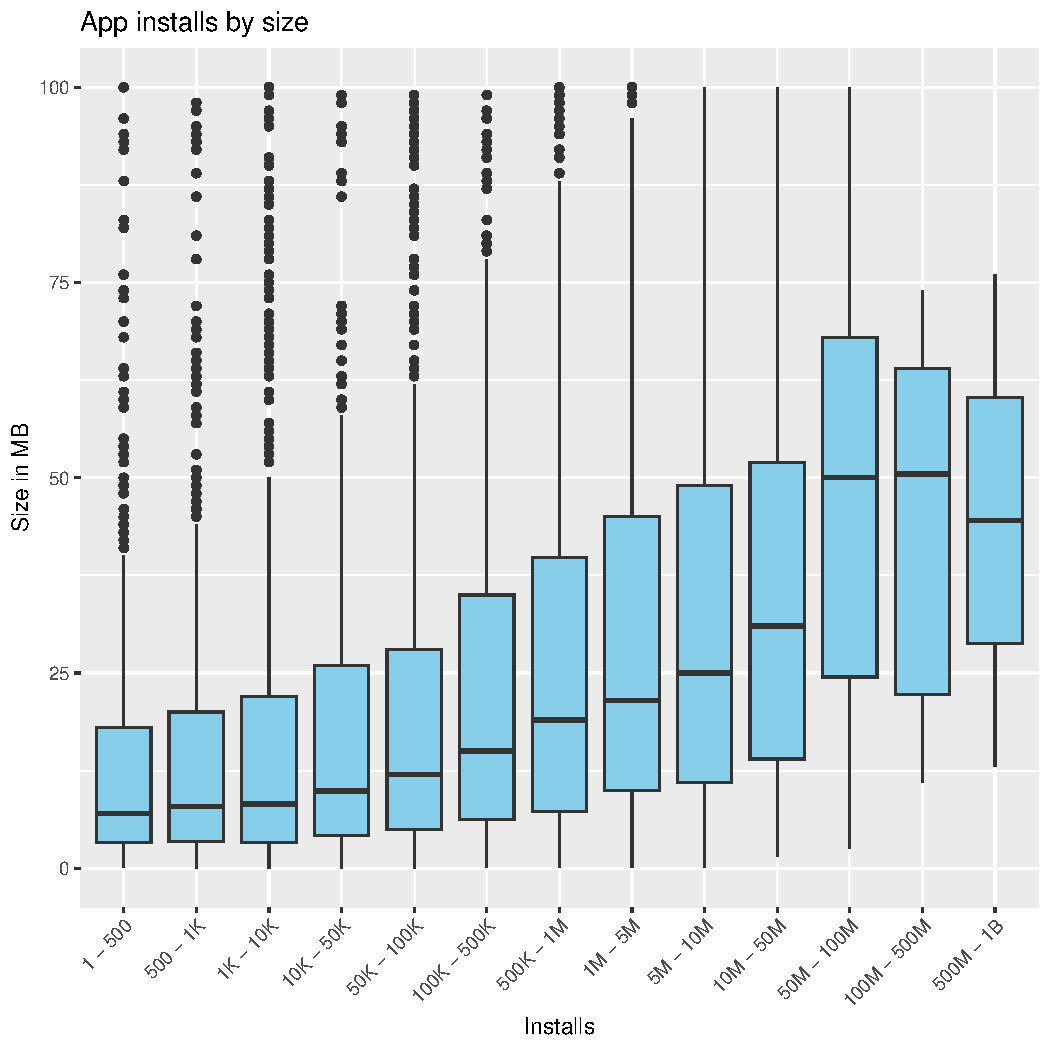
\includegraphics[width=0.75\linewidth]{C:/Users/Lewis/DataspellProjects/DataVis/Assignment/RNW/figures/installsBySizeThresholds-1} 

}

\caption[Boxplot of app size distributions across install thresholds]{Boxplot of app size distributions across install thresholds}\label{fig:installsBySizeThresholds}
\end{figure}

\end{knitrout}

\begin{knitrout}
\definecolor{shadecolor}{rgb}{0.969, 0.969, 0.969}\color{fgcolor}\begin{kframe}
\begin{alltt}
\hlstd{doesNotVary} \hlkwb{<-} \hlstd{dataDf} \hlopt
\hlcom{# Grab non-varying sizes by filtering 0 out, }
\hlcom{# then grab the first eight factor levels.}
\hlkwd{filter}\hlstd{(numSize} \hlopt{!=} \hlstr{"0"} \hlopt{&} \hlstd{installThresholds} \hlopt \hlkwd{c}\hlstd{(}\hlstr{"1 - 500"}\hlstd{,}
\hlstr{"500 - 1K"}\hlstd{,} \hlstr{"1K - 10K"}\hlstd{,}
\hlstr{"10K - 50K"}\hlstd{,} \hlstr{"50K - 100K"}\hlstd{,} \hlstr{"100K - 500K"}\hlstd{,}
\hlstr{"500K - 1M"}\hlstd{))}

\hlkwd{ggplot}\hlstd{(doesNotVary,} \hlkwd{aes}\hlstd{(}\hlkwc{x} \hlstd{= numSize))} \hlopt{+}
    \hlkwd{geom_histogram}\hlstd{(}\hlkwc{fill} \hlstd{=} \hlstr{"purple"}\hlstd{,} \hlkwc{color} \hlstd{=} \hlstr{"black"}\hlstd{,} \hlkwc{binwidth} \hlstd{=} \hlnum{4}\hlstd{)} \hlopt{+}
    \hlkwd{labs}\hlstd{(}\hlkwc{title} \hlstd{=} \hlstr{"Histogram of size distribution (1 - 1M installs)"}\hlstd{,}
         \hlkwc{x} \hlstd{=} \hlstr{"Size (in MB)"}\hlstd{,} \hlkwc{y} \hlstd{=} \hlstr{"Amount of apps"}\hlstd{)} \hlopt{+}
    \hlkwd{theme_minimal}\hlstd{()} \hlopt{+}
    \hlkwd{theme}\hlstd{(}\hlkwc{axis.text.x} \hlstd{=} \hlkwd{element_text}\hlstd{(}\hlkwc{angle} \hlstd{=} \hlnum{45}\hlstd{,} \hlkwc{hjust} \hlstd{=} \hlnum{1}\hlstd{))} \hlopt{+}
    \hlkwd{facet_wrap}\hlstd{(}\hlopt{~}\hlstd{installThresholds,} \hlkwc{ncol} \hlstd{=} \hlnum{3}\hlstd{)}
\end{alltt}
\end{kframe}\begin{figure}[H]

{\centering 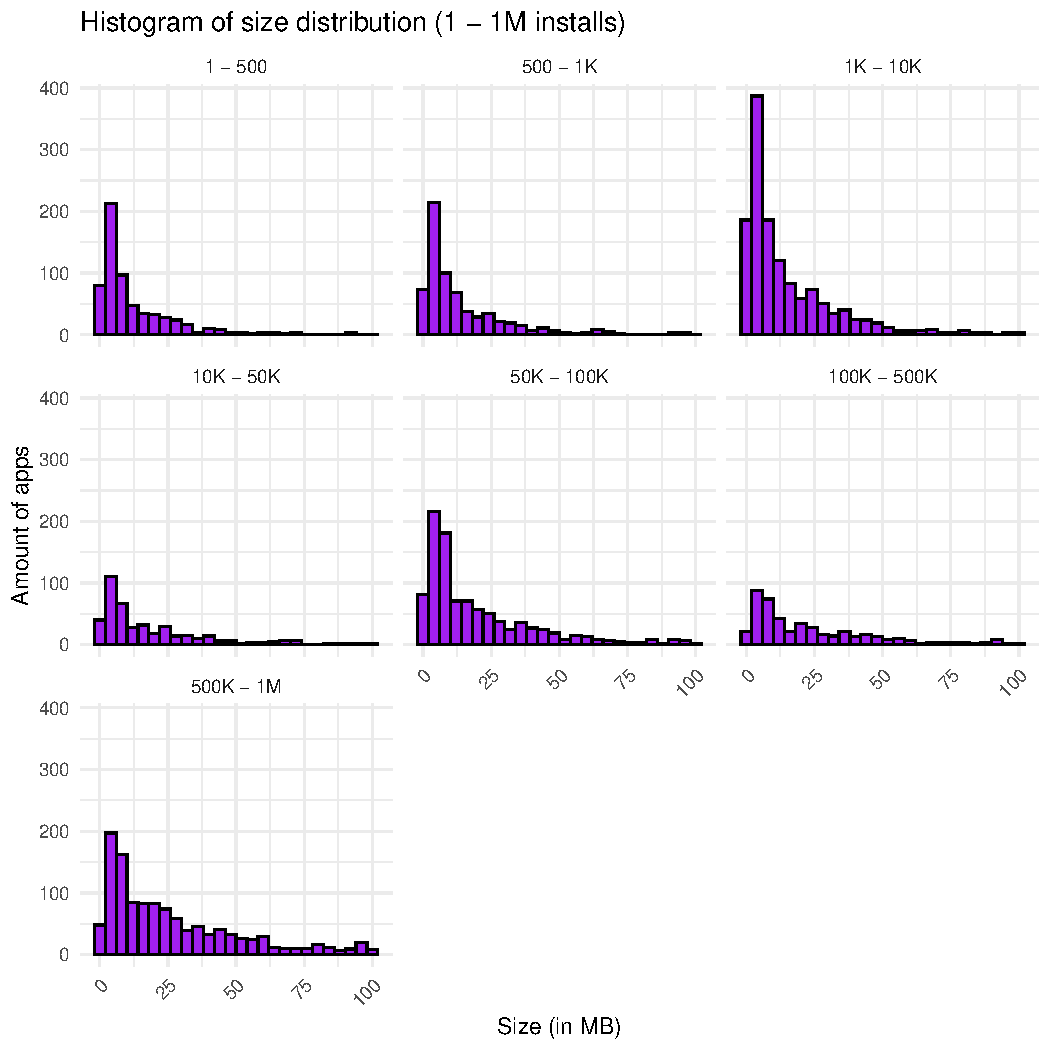
\includegraphics[width=0.75\linewidth]{C:/Users/Lewis/DataspellProjects/DataVis/Assignment/RNW/figures/halfInstallsByNumSize1-1} 

}

\caption[Size distribution across apps between 1 and 1 million installs]{Size distribution across apps between 1 and 1 million installs}\label{fig:halfInstallsByNumSize1}
\end{figure}

\end{knitrout}


\begin{knitrout}
\definecolor{shadecolor}{rgb}{0.969, 0.969, 0.969}\color{fgcolor}\begin{kframe}
\begin{alltt}
\hlstd{doesNotVary} \hlkwb{<-} \hlstd{dataDf} \hlopt
\hlcom{# Grab the other factor levels.}
\hlkwd{filter}\hlstd{(numSize} \hlopt{!=} \hlstr{"0"} \hlopt{&} \hlstd{installThresholds} \hlopt \hlkwd{c}\hlstd{(}\hlstr{"1M - 5M"}\hlstd{,}
\hlstr{"5M - 10M"}\hlstd{,} \hlstr{"10M - 50M"}\hlstd{,} \hlstr{"50M - 100M"}\hlstd{,}
\hlstr{"100M - 500M"}\hlstd{,} \hlstr{"500M - 1B"}\hlstd{))}

\hlkwd{ggplot}\hlstd{(doesNotVary,} \hlkwd{aes}\hlstd{(}\hlkwc{x} \hlstd{= numSize))} \hlopt{+}
    \hlkwd{geom_histogram}\hlstd{(}\hlkwc{fill} \hlstd{=} \hlstr{"purple"}\hlstd{,} \hlkwc{color} \hlstd{=} \hlstr{"black"}\hlstd{,} \hlkwc{binwidth} \hlstd{=} \hlnum{4}\hlstd{)} \hlopt{+}
    \hlkwd{labs}\hlstd{(}\hlkwc{x} \hlstd{=} \hlstr{"Size (in MB)"}\hlstd{,} \hlkwc{y} \hlstd{=} \hlstr{"Amount of apps"}\hlstd{,}
        \hlkwc{title} \hlstd{=} \hlstr{"Histogram of size distribution (1M - 1B installs)"}\hlstd{)} \hlopt{+}
    \hlkwd{theme_minimal}\hlstd{()} \hlopt{+}
    \hlkwd{theme}\hlstd{(}\hlkwc{axis.text.x} \hlstd{=} \hlkwd{element_text}\hlstd{(}\hlkwc{angle} \hlstd{=} \hlnum{45}\hlstd{,} \hlkwc{hjust} \hlstd{=} \hlnum{1}\hlstd{))} \hlopt{+}
    \hlkwd{facet_wrap}\hlstd{(}\hlopt{~}\hlstd{installThresholds,} \hlkwc{ncol} \hlstd{=} \hlnum{2}\hlstd{)}
\end{alltt}
\end{kframe}\begin{figure}[H]

{\centering 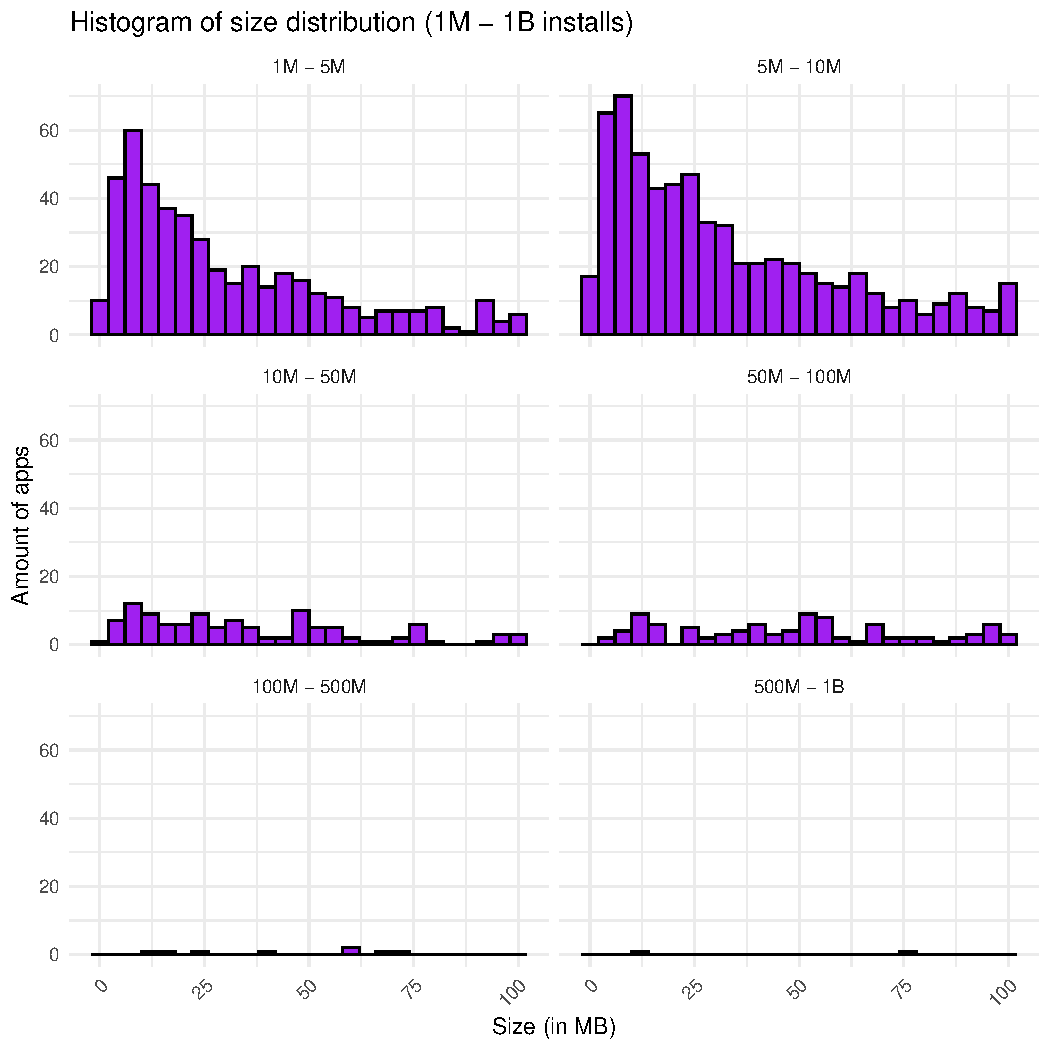
\includegraphics[width=0.75\linewidth]{C:/Users/Lewis/DataspellProjects/DataVis/Assignment/RNW/figures/halfInstallsByNumSize2-1} 

}

\caption[Size distribution across apps between 1 million and 1 billion installs]{Size distribution across apps between 1 million and 1 billion installs}\label{fig:halfInstallsByNumSize2}
\end{figure}

\end{knitrout}

\begin{knitrout}
\definecolor{shadecolor}{rgb}{0.969, 0.969, 0.969}\color{fgcolor}\begin{kframe}
\begin{alltt}
\hlstd{installsSize} \hlkwb{<-} \hlstd{installsSize} \hlopt
    \hlkwd{group_by}\hlstd{(installThresholds)} \hlopt
    \hlkwd{summarise}\hlstd{(}\hlkwc{avgSize} \hlstd{=} \hlkwd{mean}\hlstd{(numSize))}

\hlkwd{ggplot}\hlstd{(installsSize,} \hlkwd{aes}\hlstd{(}\hlkwc{x} \hlstd{= avgSize,} \hlkwc{y} \hlstd{= installThresholds,}
                         \hlkwc{fill} \hlstd{= installThresholds))} \hlopt{+}
    \hlkwd{geom_bar}\hlstd{(}\hlkwc{stat} \hlstd{=} \hlstr{"summary"}\hlstd{,} \hlkwc{fun} \hlstd{= mean)} \hlopt{+}
    \hlkwd{geom_text}\hlstd{(}\hlkwd{aes}\hlstd{(}\hlkwc{label} \hlstd{=} \hlkwd{round}\hlstd{(avgSize,} \hlnum{3}\hlstd{)),}
              \hlkwc{position} \hlstd{=} \hlkwd{position_stack}\hlstd{(}\hlkwc{vjust} \hlstd{=} \hlnum{0.5}\hlstd{))} \hlopt{+}
    \hlkwd{labs}\hlstd{(}\hlkwc{title} \hlstd{=} \hlstr{"Average size of apps by install threshold"}\hlstd{,}
         \hlkwc{x} \hlstd{=} \hlstr{"Size in MB"}\hlstd{,} \hlkwc{y} \hlstd{=} \hlstr{"Installs"}\hlstd{)} \hlopt{+}
    \hlkwd{theme}\hlstd{(}\hlkwc{axis.text.x} \hlstd{=} \hlkwd{element_text}\hlstd{(}\hlkwc{angle} \hlstd{=} \hlnum{45}\hlstd{,} \hlkwc{hjust} \hlstd{=} \hlnum{1}\hlstd{),}
          \hlkwc{legend.position} \hlstd{=} \hlstr{"none"}\hlstd{)}
\end{alltt}
\end{kframe}\begin{figure}[H]

{\centering 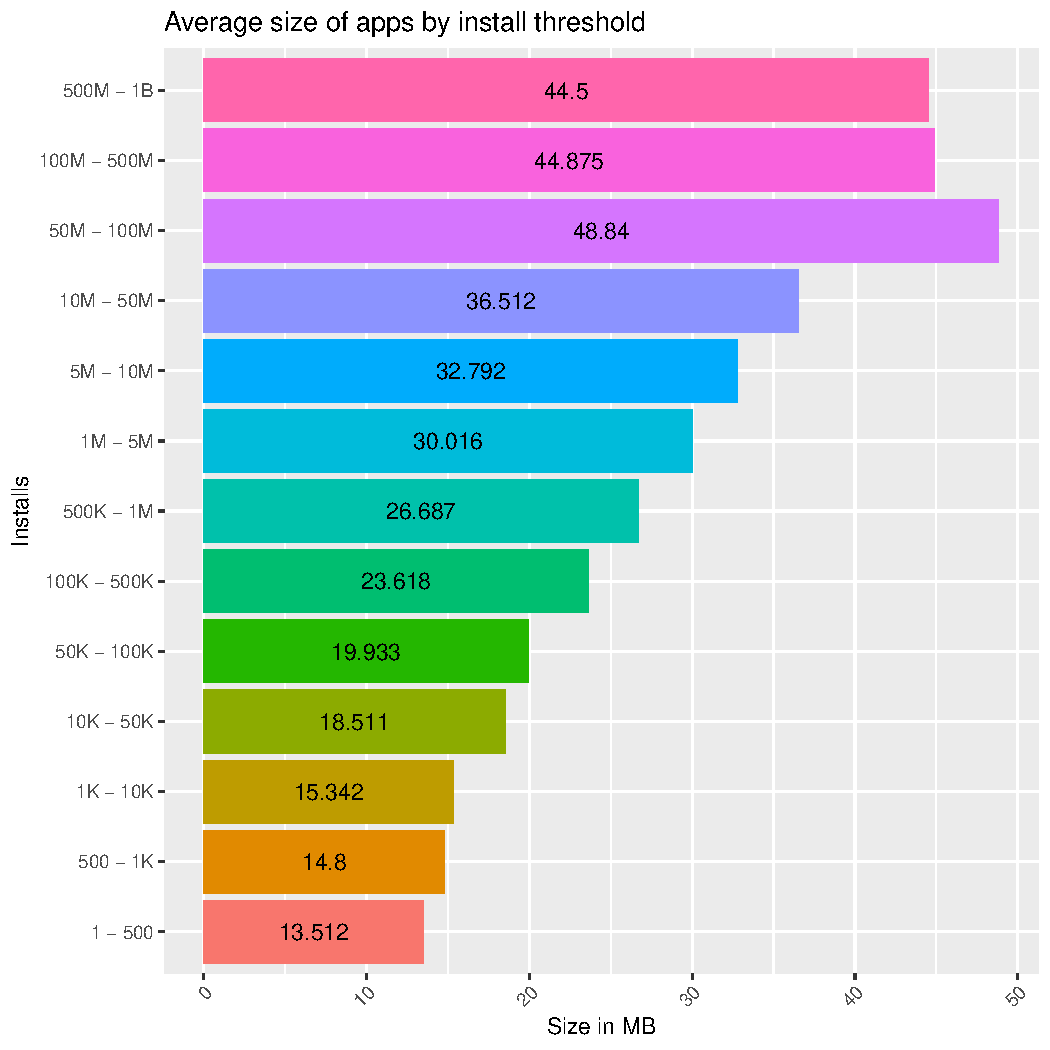
\includegraphics[width=0.75\linewidth]{C:/Users/Lewis/DataspellProjects/DataVis/Assignment/RNW/figures/avgSizeInstall-1} 

}

\caption[Average size of apps by install threshold]{Average size of apps by install threshold}\label{fig:avgSizeInstall}
\end{figure}

\end{knitrout}

Interestingly, we can observe a mostly positive correlation between app size and install count,
with the average sizes of apps mostly increasing by small amounts, except for apps with between
100 million and 1 billion downloads, which both sit around the 44/45 megabyte size on average. 
This suggests that it is important to ensure that while apps do have a variety of features that would
increase their size, it is important to optimise it where possible due to the limited storage space available 
on mobile devices that could cause the user to uninstall apps in favour of others.



\chapter{Summary and conclusion}
% Put the chapter name in the header.
\markboth{Summary and conclusion}{}



\section{Summary}
\begin{itemize}
    \item Is there a positive correlation between the average review score of an app and its install count? 
    \begin{itemize}
        \item Expected: Yes, as it is harder to weigh the average down when the volume
        of installs increases.
        \item Actual: Yes, there is a positive correlation between the two.
    \end{itemize}
    \item Which category of app has the highest review score on average?
    \begin{itemize}
        \item Expected: Games are likely to have the highest review scores from users
        enjoying their experiences.
        \item Actual: Events apps have the highest review score on average due to a low sample size.
        \item Of the top five categories, however, Games are rated the highest.
    \end{itemize}
    \item What is the distribution of prices? Are there certain prices used by many apps?
    \begin{itemize}
        \item Expected: If an app is not free, it would likely be under \$3 to ensure
        people buy it.
        \item Actual: The majority of apps are priced at \$2.99, \$0.99 or \$4.99.
    \end{itemize}
    \item Do paid apps receive higher or lower review score on average?
    \begin{itemize}
        \item Expected: No, as users may be more harsh with their reviews if they paid
        for the app.
        \item Actual: Paid apps actually do receive higher average ratings, perhaps due to users instead being more
                      forgiving of products that they paid money for.
    \end{itemize}
    \item Is there a correlation between an app's content rating and it's review score?
    \begin{itemize}
        \item Expected: Yes, with adult apps likely being higher rated because children
        would be unlikely to have accounts.
        \item Actual: Yes, though it is somewhat minor. Expectations were defied due to "Adults only" apps
                      actually being the lowest rated on average.
    \end{itemize}
    \item Does app size play a role in install count?
    \begin{itemize}
        \item Expected: Yes, as users would likely not want to download very large
        apps due to internet speeds and device storage.
        \item Actual: The data showed a positive correlation between average size and install count to a plateau of approximately 49MB.
    \end{itemize}
\end{itemize}

\section{Conclusion}

This report has analyzed a dataset of Google Play Store apps,
revealing valuable insights into app characteristics, user ratings, and trends. 
We observed the distributions of data across the dataset, revealing trends in 
review scores and install counts with categories, prices, age ratings and app size, and showing 
how they may not be as one would expect.
Overall, this exploration of the Google Play Store data provides great benefit to
app developers and users alike; developers can leverage these insights to 
identify key focus points in the development process, such as tailoring their apps to be for certain age 
groups or pricing them at certain costs, and for users, understanding these
trends can inform their app selection process, leading them towards apps that better meet their needs.

\printbibliography{}

\end{document}


